%!TEX root = ../2019_06_04-HATS-LPC-JEC.tex

\begin{frame}
	\begin{block}{}
        \begin{center}
            \shadowoffset{2pt}
            \shadowcolor{CUGold}
            \shadowtext{{\fontsize{30}{60}\selectfont \textbf{\textcolor{black}{Backup Slides}}}}
            \vspace{1.5mm}
        \end{center}
    \end{block}
\end{frame}
%---------------------------------------------------------------------------------------------------------------------------------------
{
\setbeamercolor{background canvas}{bg=}
\includepdf[pages=1-6]{hats_pileup2018-backup_slides.pdf}
}
\addtocounter{framenumber}{6}

\begin{comment}
\subsection{How do we guarantee we are correcting what we think we are correcting?}
\frame{
	\frametitle{How do we guarantee we are correcting what we think we are correcting?}

	Pileup - match same jet without PU to jet with PU. Litterally the only difference is the additional energy due to PU. Can't be anything else...maybe small matching uncertainty

	L2L3 MCTruth - We in in jet pt as well as ref pt and eta so that we are independent of the jet pt spectrum. Otherwise our corrections would only be valid for sampels with the same pt spectrum (because the average energies would be different)
	
	L5 - second order correction to L2L3, but binned in flavor. Same type of correction though (response based). Again, binned in jet pt, ref pt, and eta.
	
	L2L3Res - make sure that we are measuring the dijet case by using an $\alpha<0.3$ cut. Then we extrapolate to the $\alpha=0$ value. This means that the pt of any third jet is really low. Then take the ratio of MC/data. Thus we are really measuring the difference of MC to data in the dijet case.
}
\end{comment}

\subsubsection*{PileUp}
\frame{
	\frametitle{Old PileUpPt (from 2013)}
	\vspace*{-0.24cm}
	\begin{columns}[T]
	\hspace*{0.3cm}\column{0.43\textwidth}
		\vspace*{-0.3cm}
		\begin{block}{}
			\begin{itemize}
				\small
				\item Old PileUpPt systematic was 100\% the difference between MC truth (V1) and Random Cone (V0)
				\begin{itemize}
					\footnotesize
					\item MC truth: effective offset inside the jet
					\item Random Cone: effective offset outside the jet
					\item Possible inside-outside differences include zero suppression, PF thresholds, calibration non-linearities etc.
				\end{itemize}		
			\end{itemize}
		\end{block}
	\column{0.6\textwidth}
	\begin{textblock}{0.5}(0.48,0.05)
	\begin{block}{}
		\begin{itemize}
			\small
			\item New PileUpPt would have been $\leq60\%$ just from global L3Residual fit and improved EE offset modeling in RD MC
		\end{itemize}
	\end{block}
	\end{textblock}
	\vspace*{0.7cm}
	\begin{myfancyblock}
		\node[anchor=south west,inner sep=0] (image) at (0,0) {%
			\hspace*{0.2cm}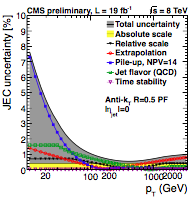
\includegraphics[width=0.48\textwidth]{images/JECUncert_Summer13_DATA_Summary_AK5PF_Eta00.png}%
			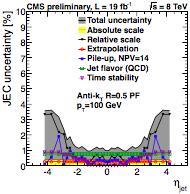
\includegraphics[width=0.48\textwidth]{images/JECUncert_Summer13_DATA_Summary_AK5PF_Pt100.png}%
		};
	\end{myfancyblock}
	\end{columns}
	\vspace*{-0.25cm}
	\begin{myfancyblock}
		\node[anchor=south west,inner sep=0] (image) at (0,0) {%
			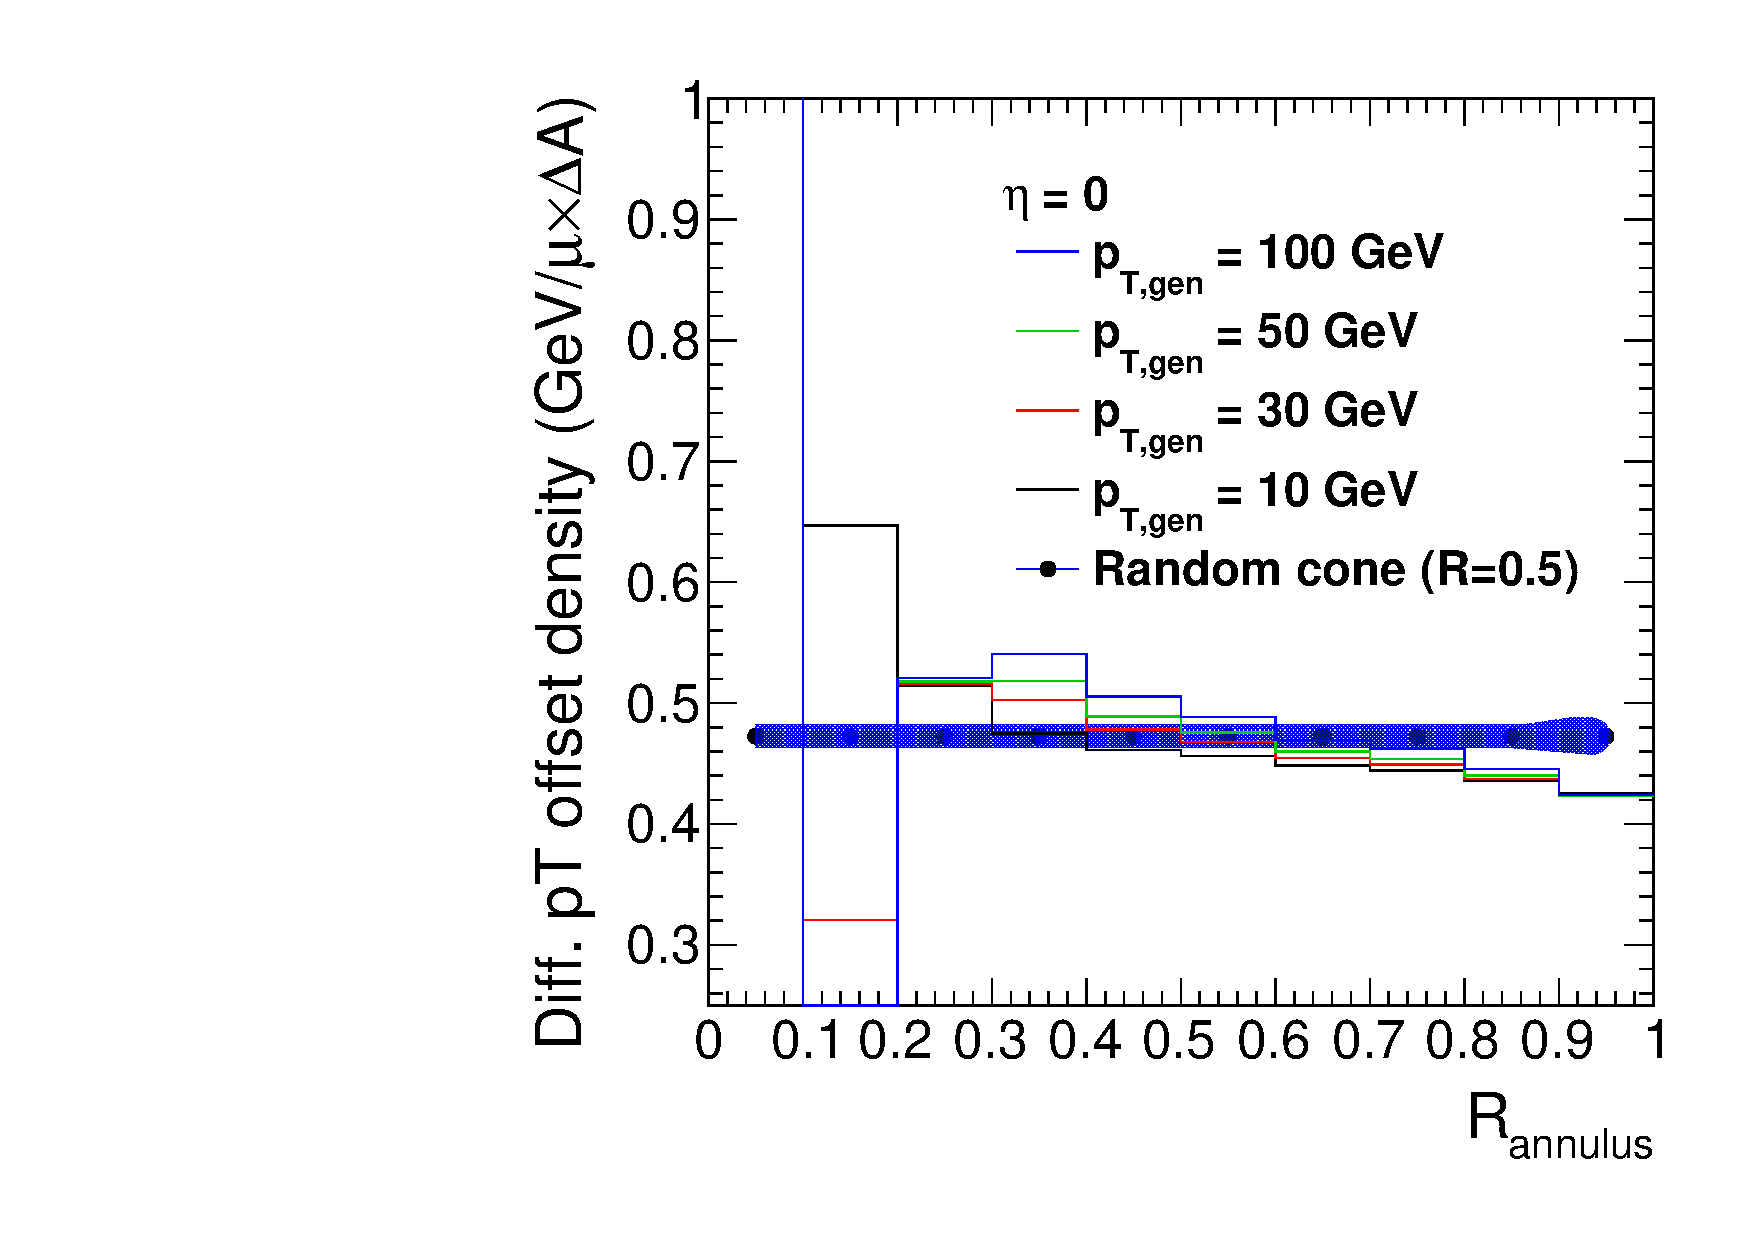
\includegraphics[width=0.25\textwidth]{images/offsetVsDeltaR_Eta00_pTOffset.pdf}%
			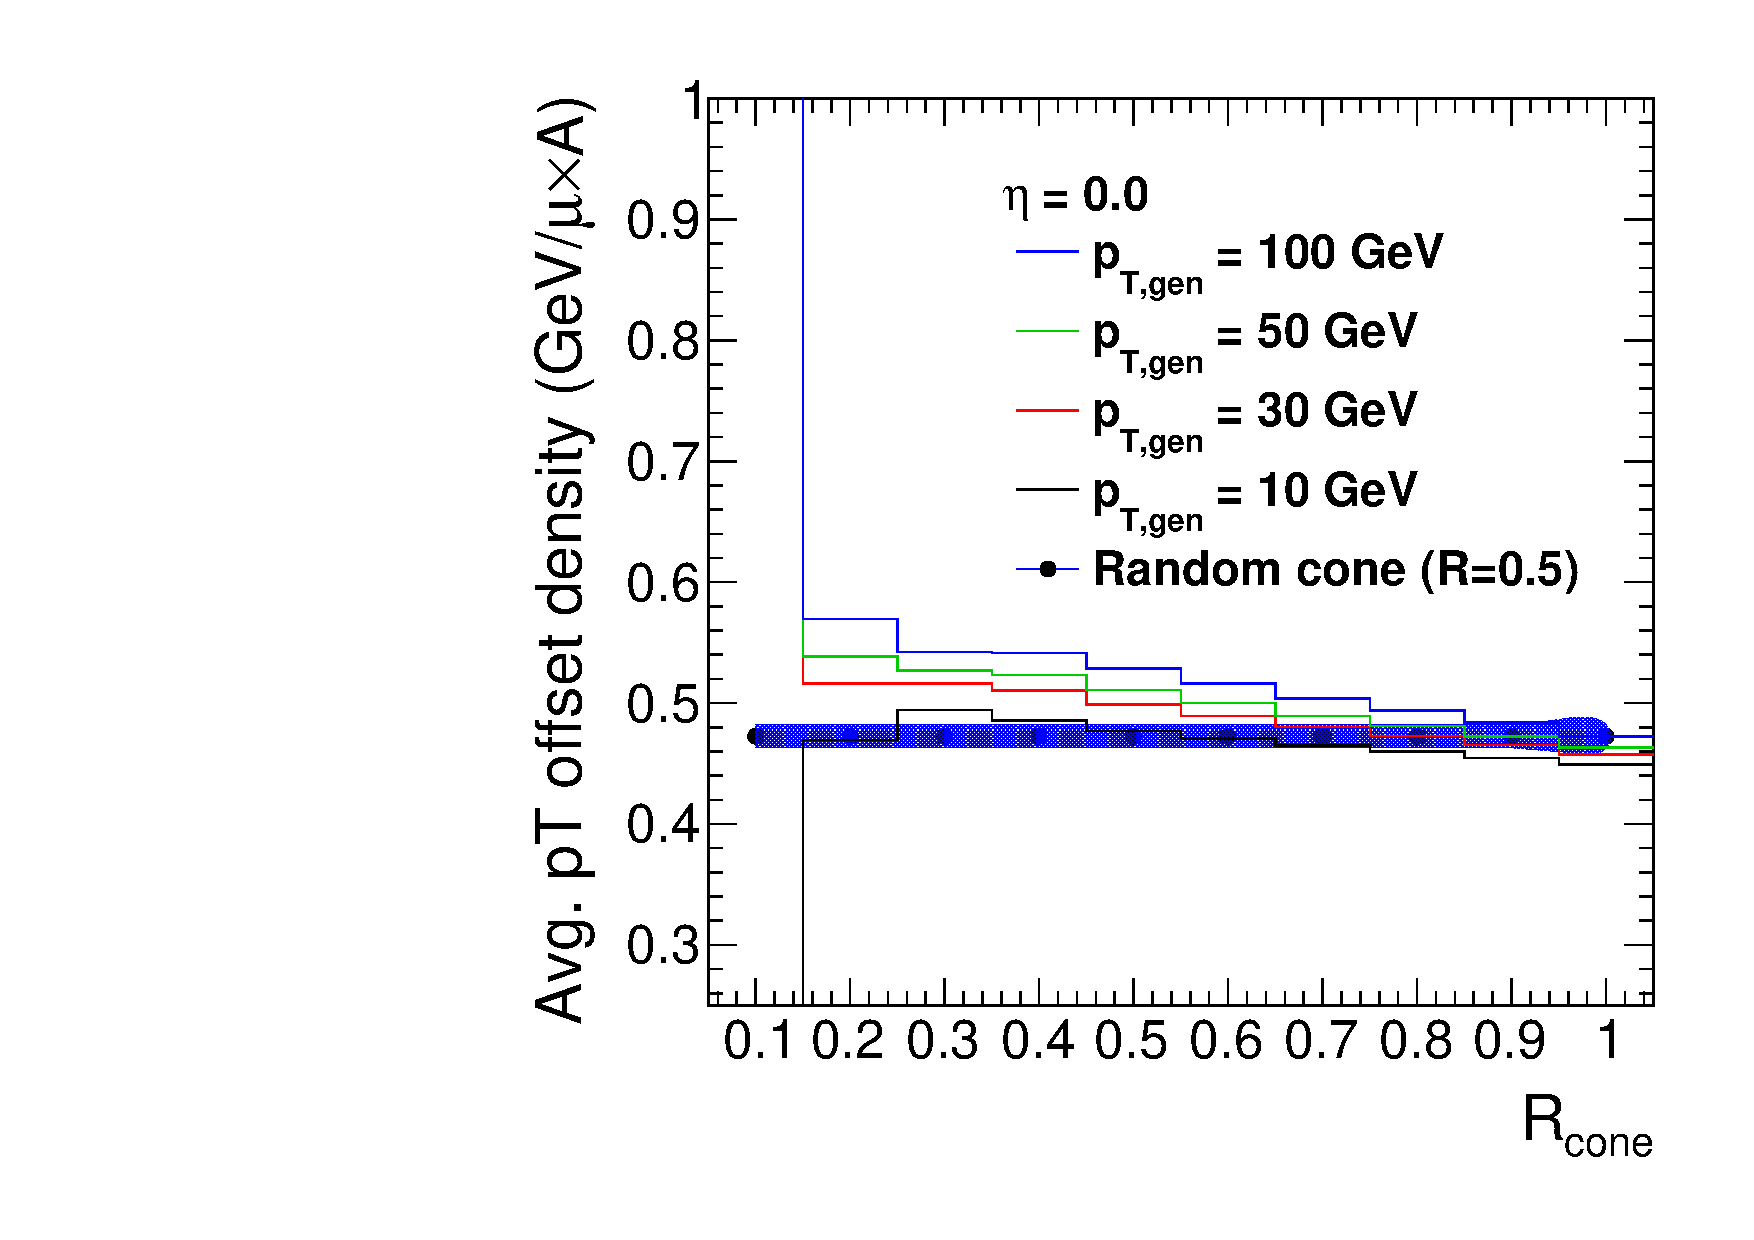
\includegraphics[width=0.25\textwidth]{images/offsetVsRcone_Eta00_pTOffset.pdf}%
			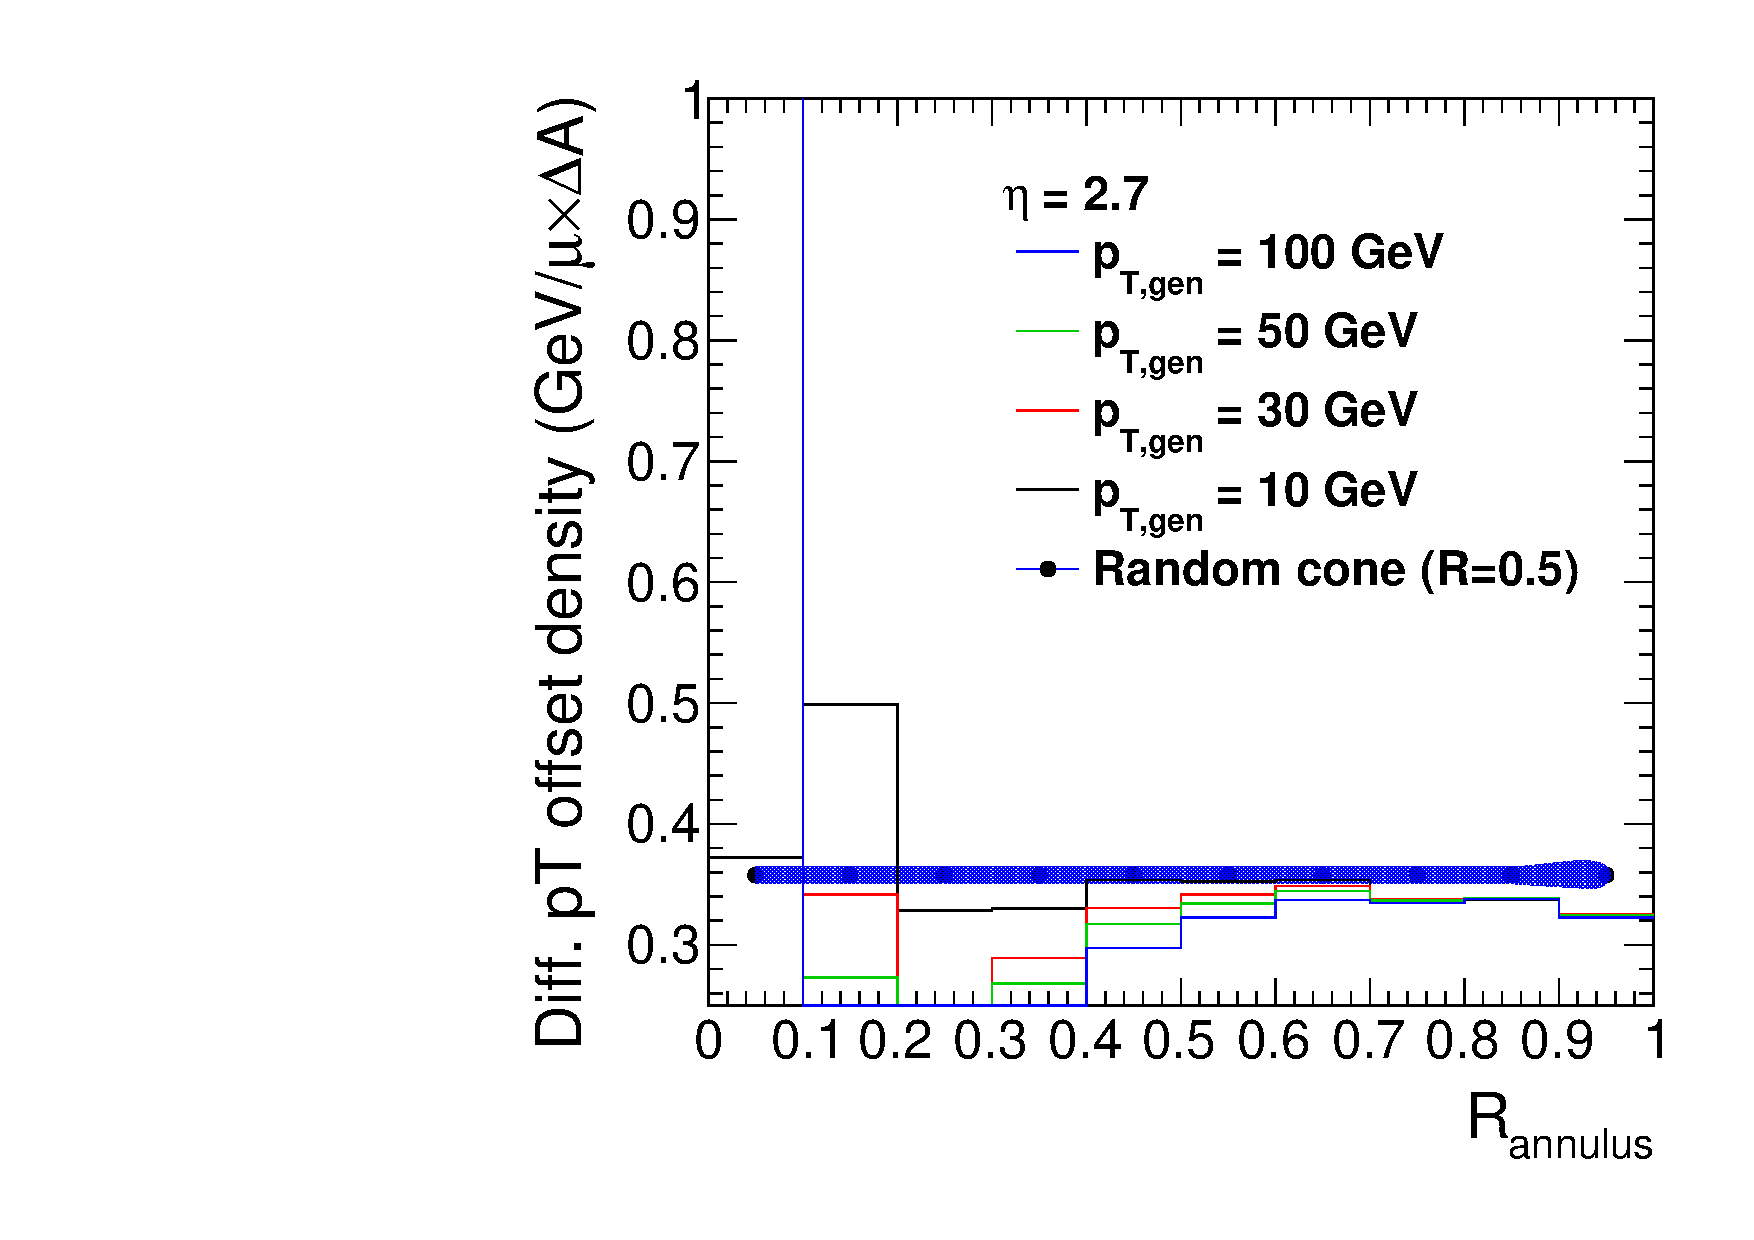
\includegraphics[width=0.25\textwidth]{images/offsetVsDeltaR_Eta27_pTOffset.pdf}%
			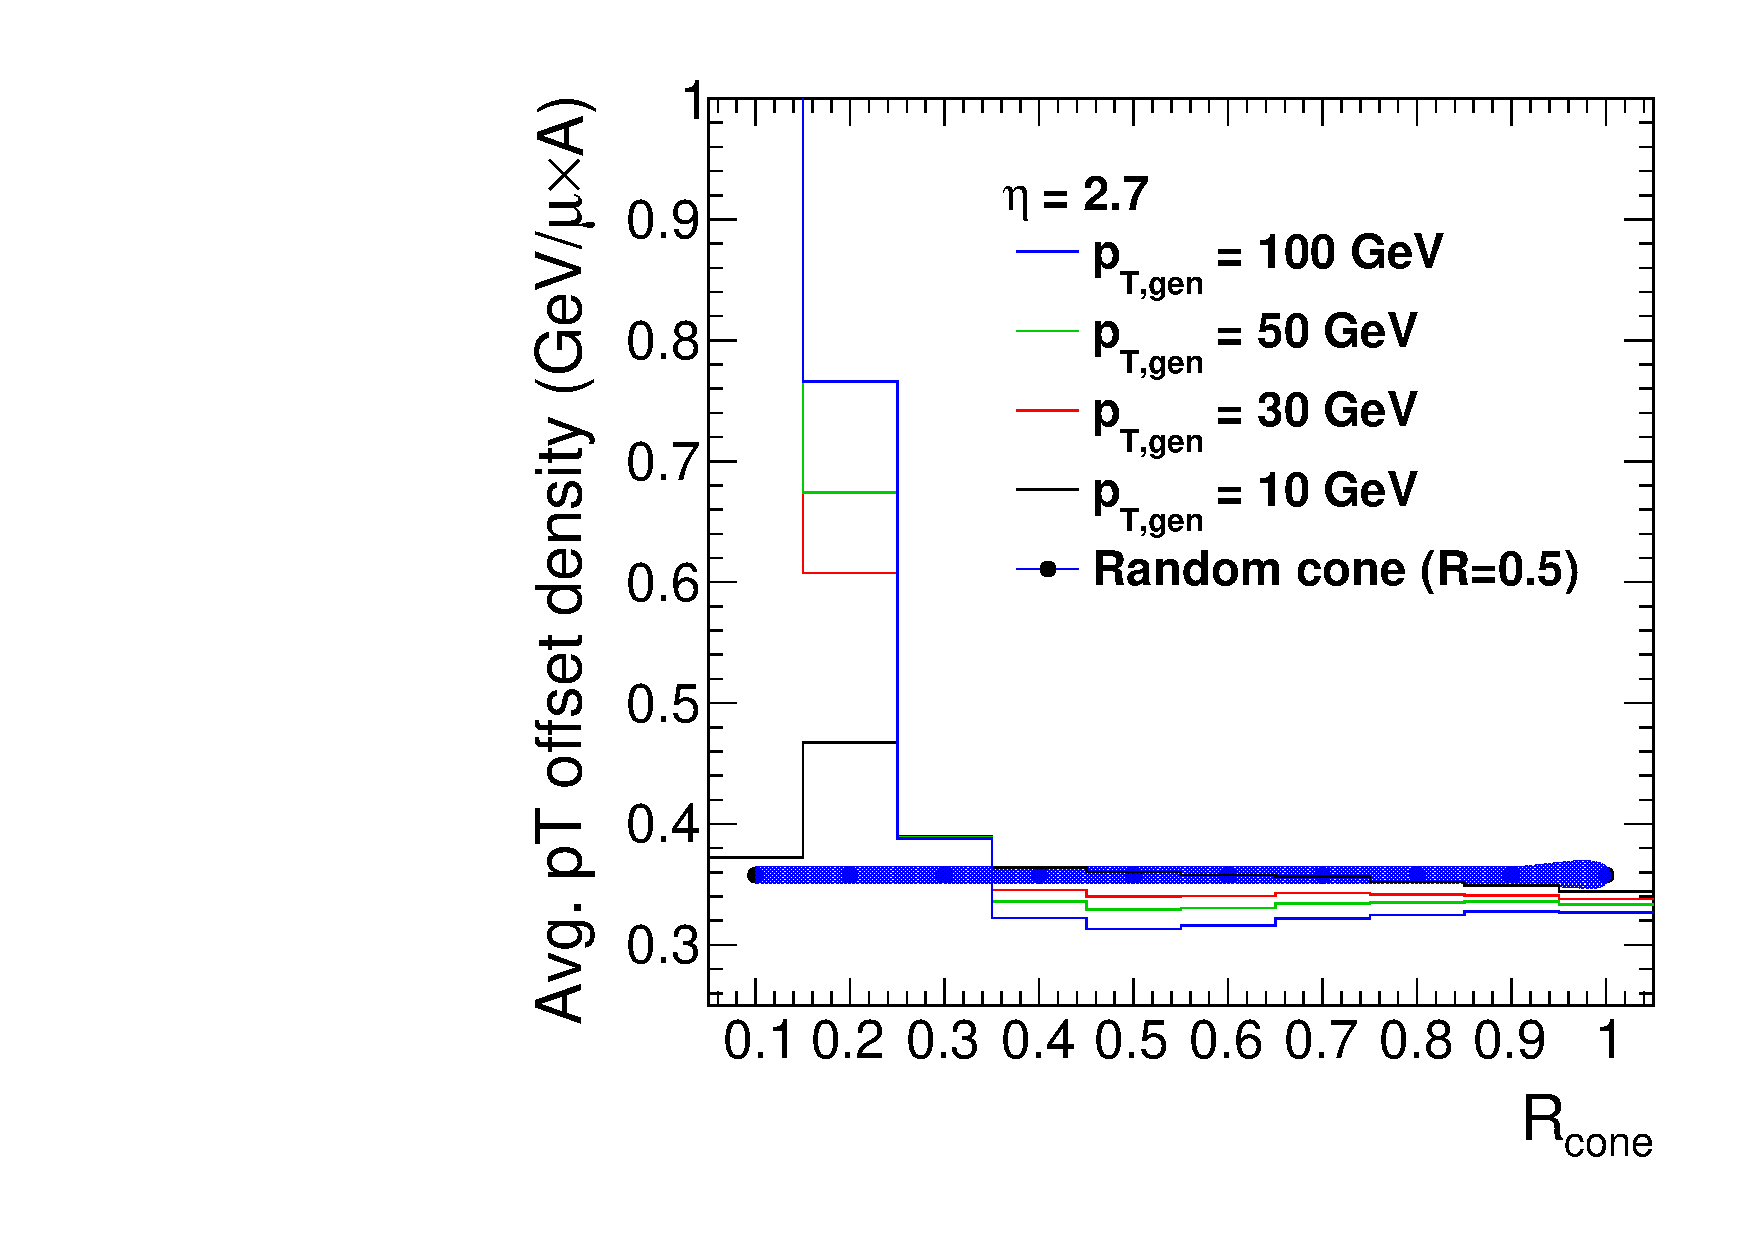
\includegraphics[width=0.25\textwidth]{images/offsetVsRcone_Eta27_pTOffset.pdf}%
		};
	\end{myfancyblock}
}
\frame{
	\frametitle{PileUpPtRef}
	\framesubtitle{AK5PFchs \& AK7PF}
	\vspace*{-0.24cm}
	\begin{block}{}
		\begin{itemize}
			\small
			\item New, more detailed treatment of pile-up uncertainties
			\item Takes into account the effective compensation of the residual offset in dijet and Z$+$jet balancing for $<\mu>=20$ (useful for $2.76\unit{TeV}$ data)
			\item Reduces uncertainties at low $p_{T}$ (relevant for top group) and $|\eta|>2$ (relevant for SMP-J)
			\item Helped in identifying pileup systematics correlations between $2.76\unit{TeV}$ and $8\unit{TeV}$ (relevant for SMP-J)
			\item L3Res only for AK5PFchs, so offset systematics in barrel grow for other algorithms
			\begin{itemize}
				\footnotesize
				\item While using AK5PFchs residuals for the other algorithms increases pileup systematics at low $p_{T}$, it also reduces the anti-correlation with high $p_{T}$
			\end{itemize}
		\end{itemize}
	\end{block}
	\vspace*{-0.1cm}
	\begin{myfancyblock}
		\node[anchor=south west,inner sep=0] (image) at (0,0) {%
			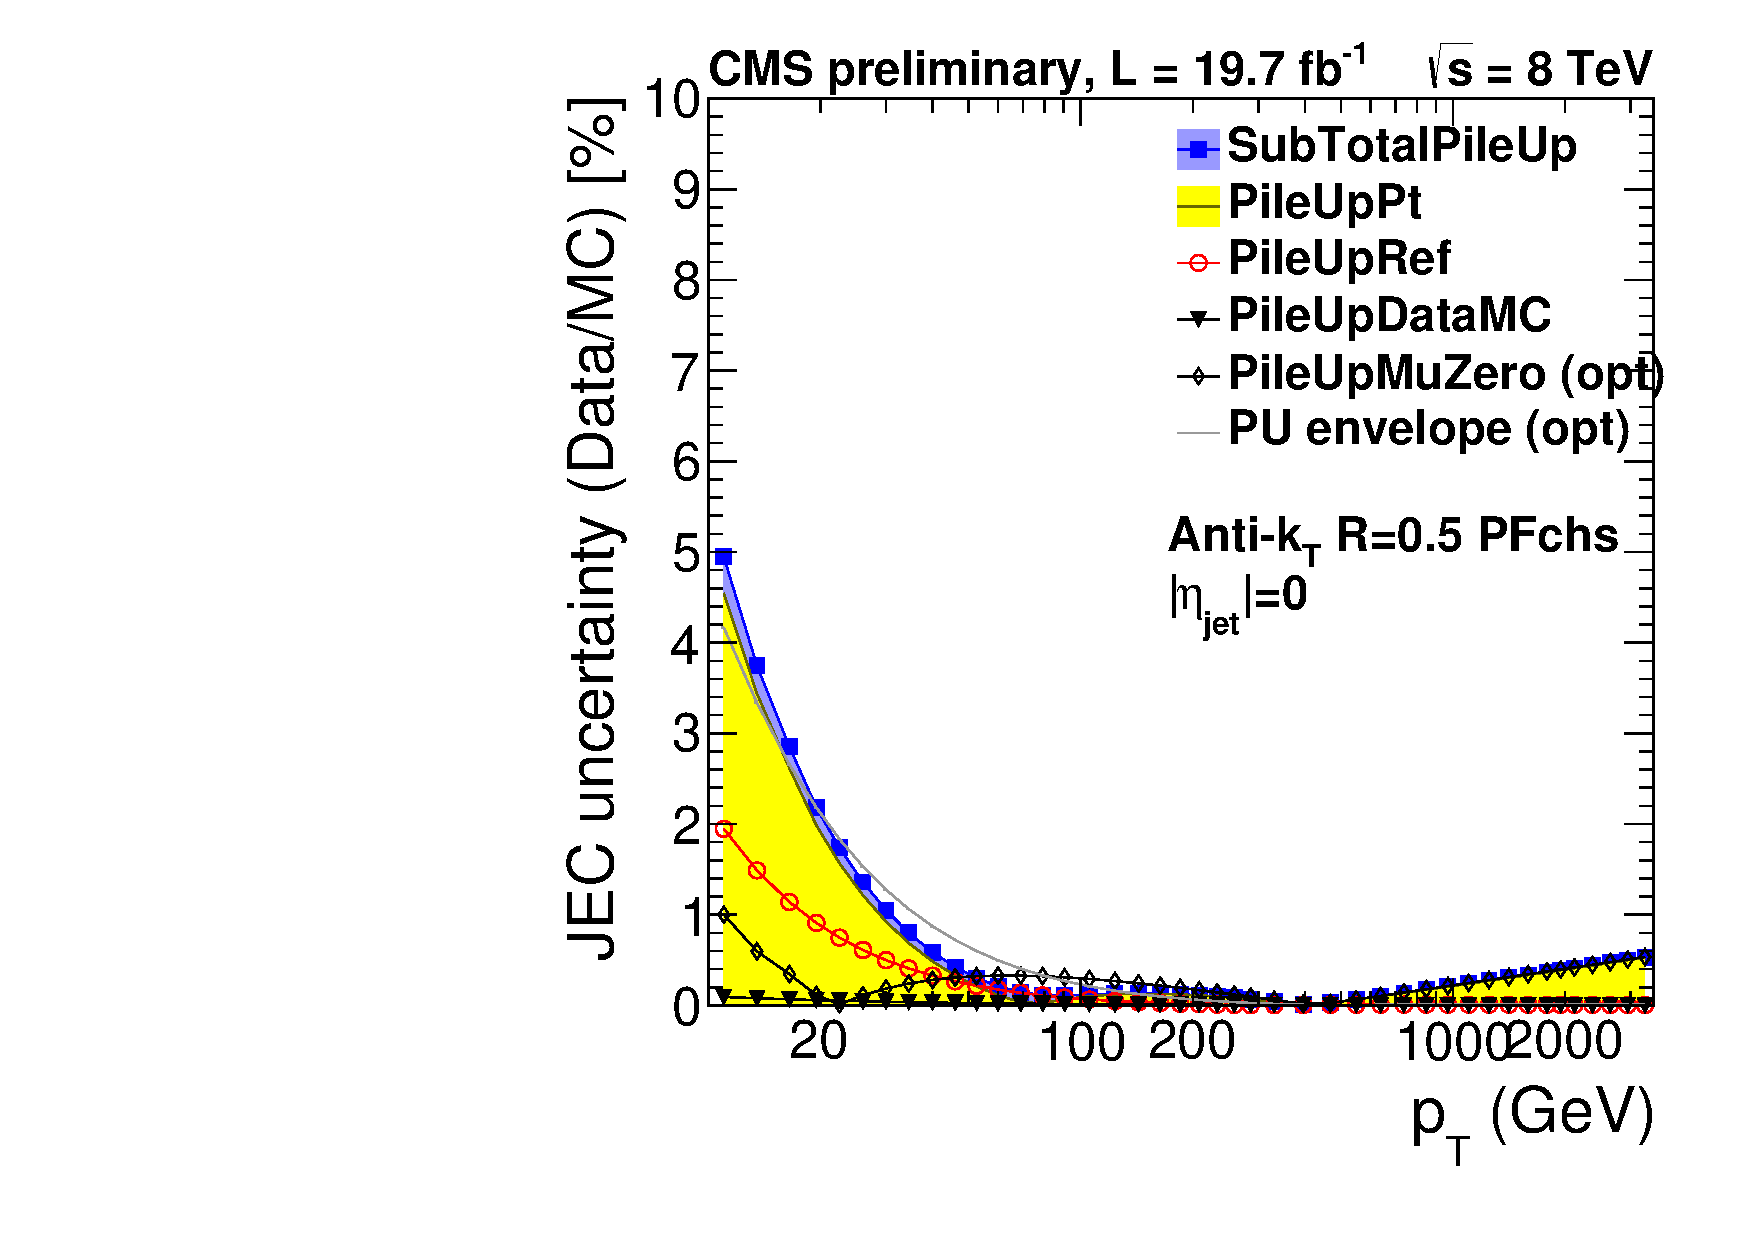
\includegraphics[width=0.25\textwidth]{images/JECUncert_PileUp_AK5PFchs_Eta00.pdf}%
			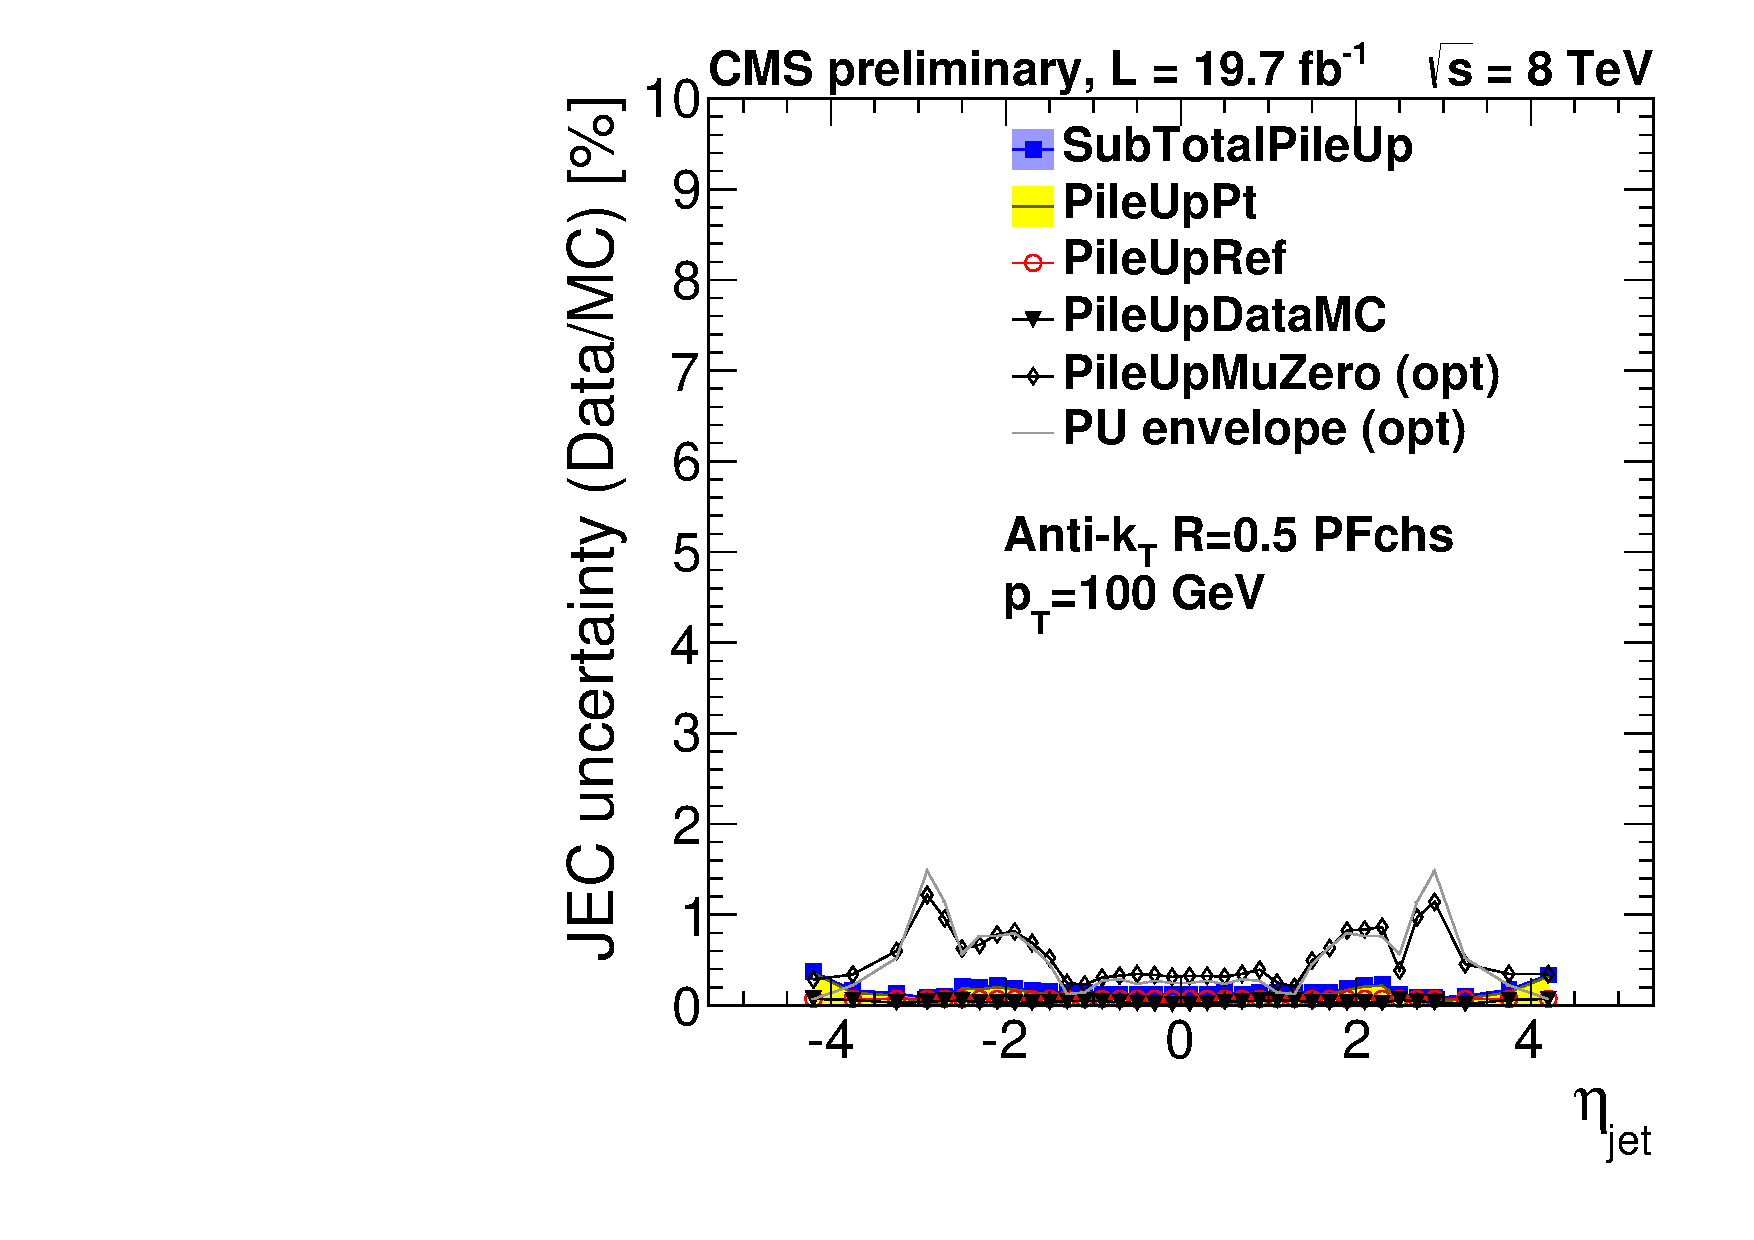
\includegraphics[width=0.25\textwidth]{images/JECUncert_PileUp_AK5PFchs_Pt100.pdf}%
			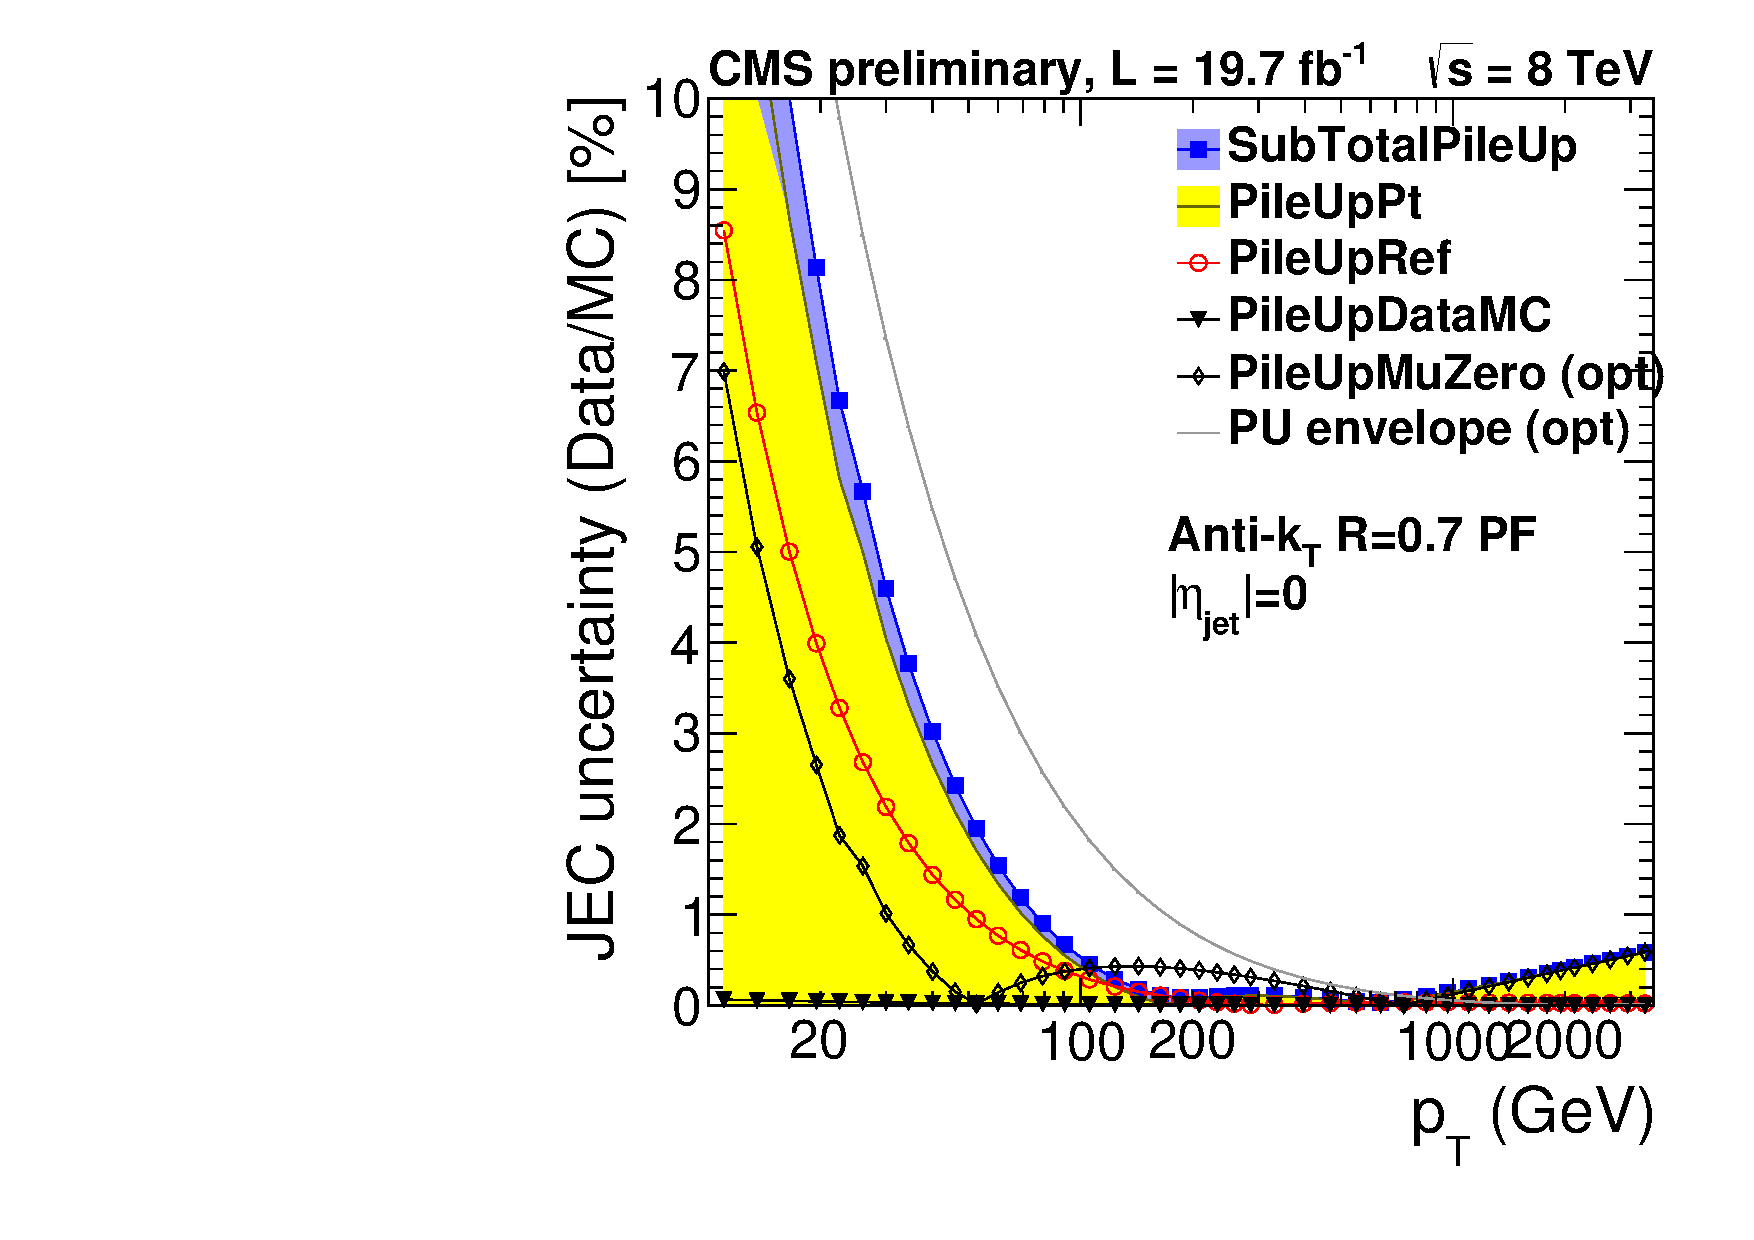
\includegraphics[width=0.25\textwidth]{images/JECUncert_PileUp_AK7PF_Eta00.pdf}%
			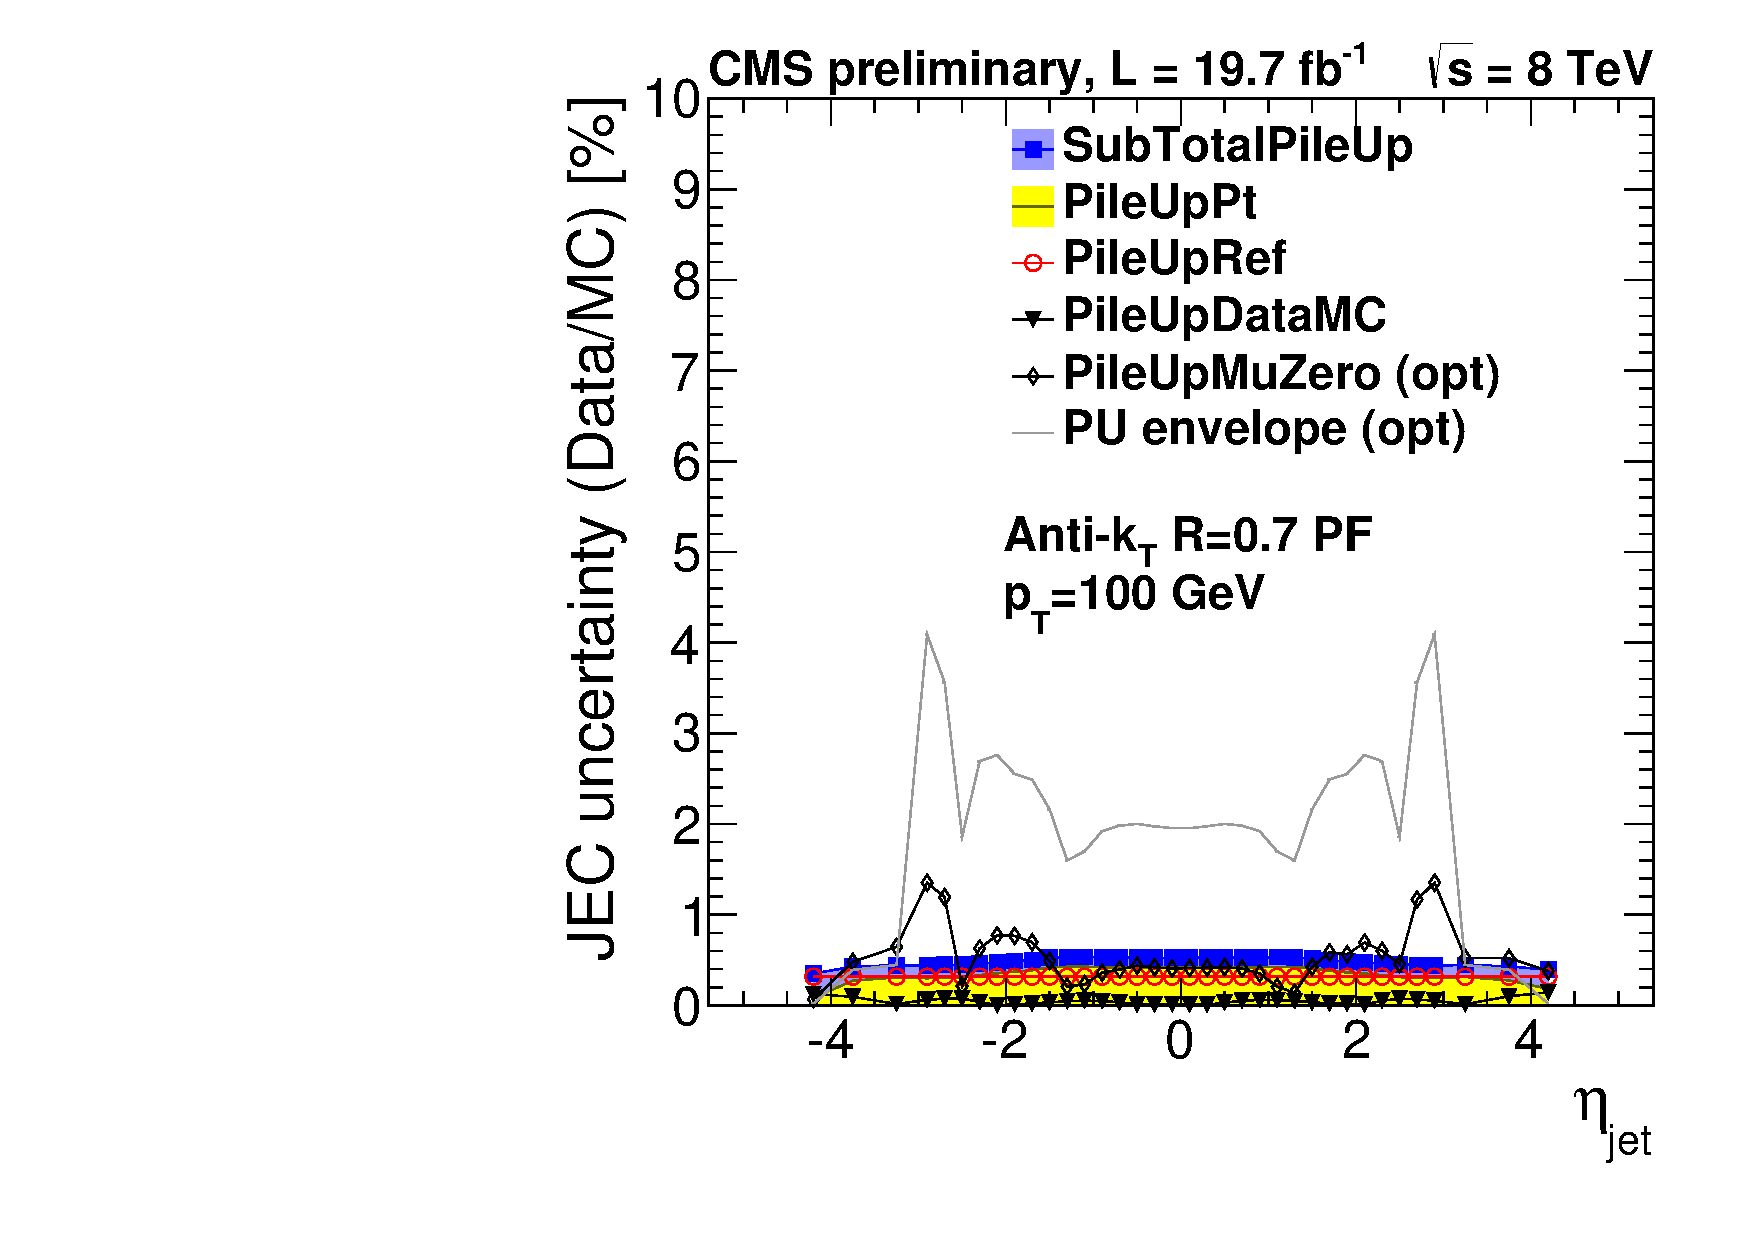
\includegraphics[width=0.25\textwidth]{images/JECUncert_PileUp_AK7PF_Pt100.pdf}%
		};
	\end{myfancyblock}
}
\frame{
	\frametitle{PileUpPt[Eta]}
	\framesubtitle{AK5PFchs \& AK7PF}
	\vspace*{-0.24cm}
	\begin{block}{}
		\begin{itemize}
			\item L2Res corrects for residual offset relative to barrel, for $<\mu>=20$ and $p_{T}=(30)60-2000\unit{GeV}$
			\item Uncertainty grows for AK7PF due to larger offset and for higher fit range $p_{T}>71\unit{GeV}$
		\end{itemize}
	\end{block}
	\begin{myfancyblock}
		\node[anchor=south west,inner sep=0] (image) at (0,0) {%
			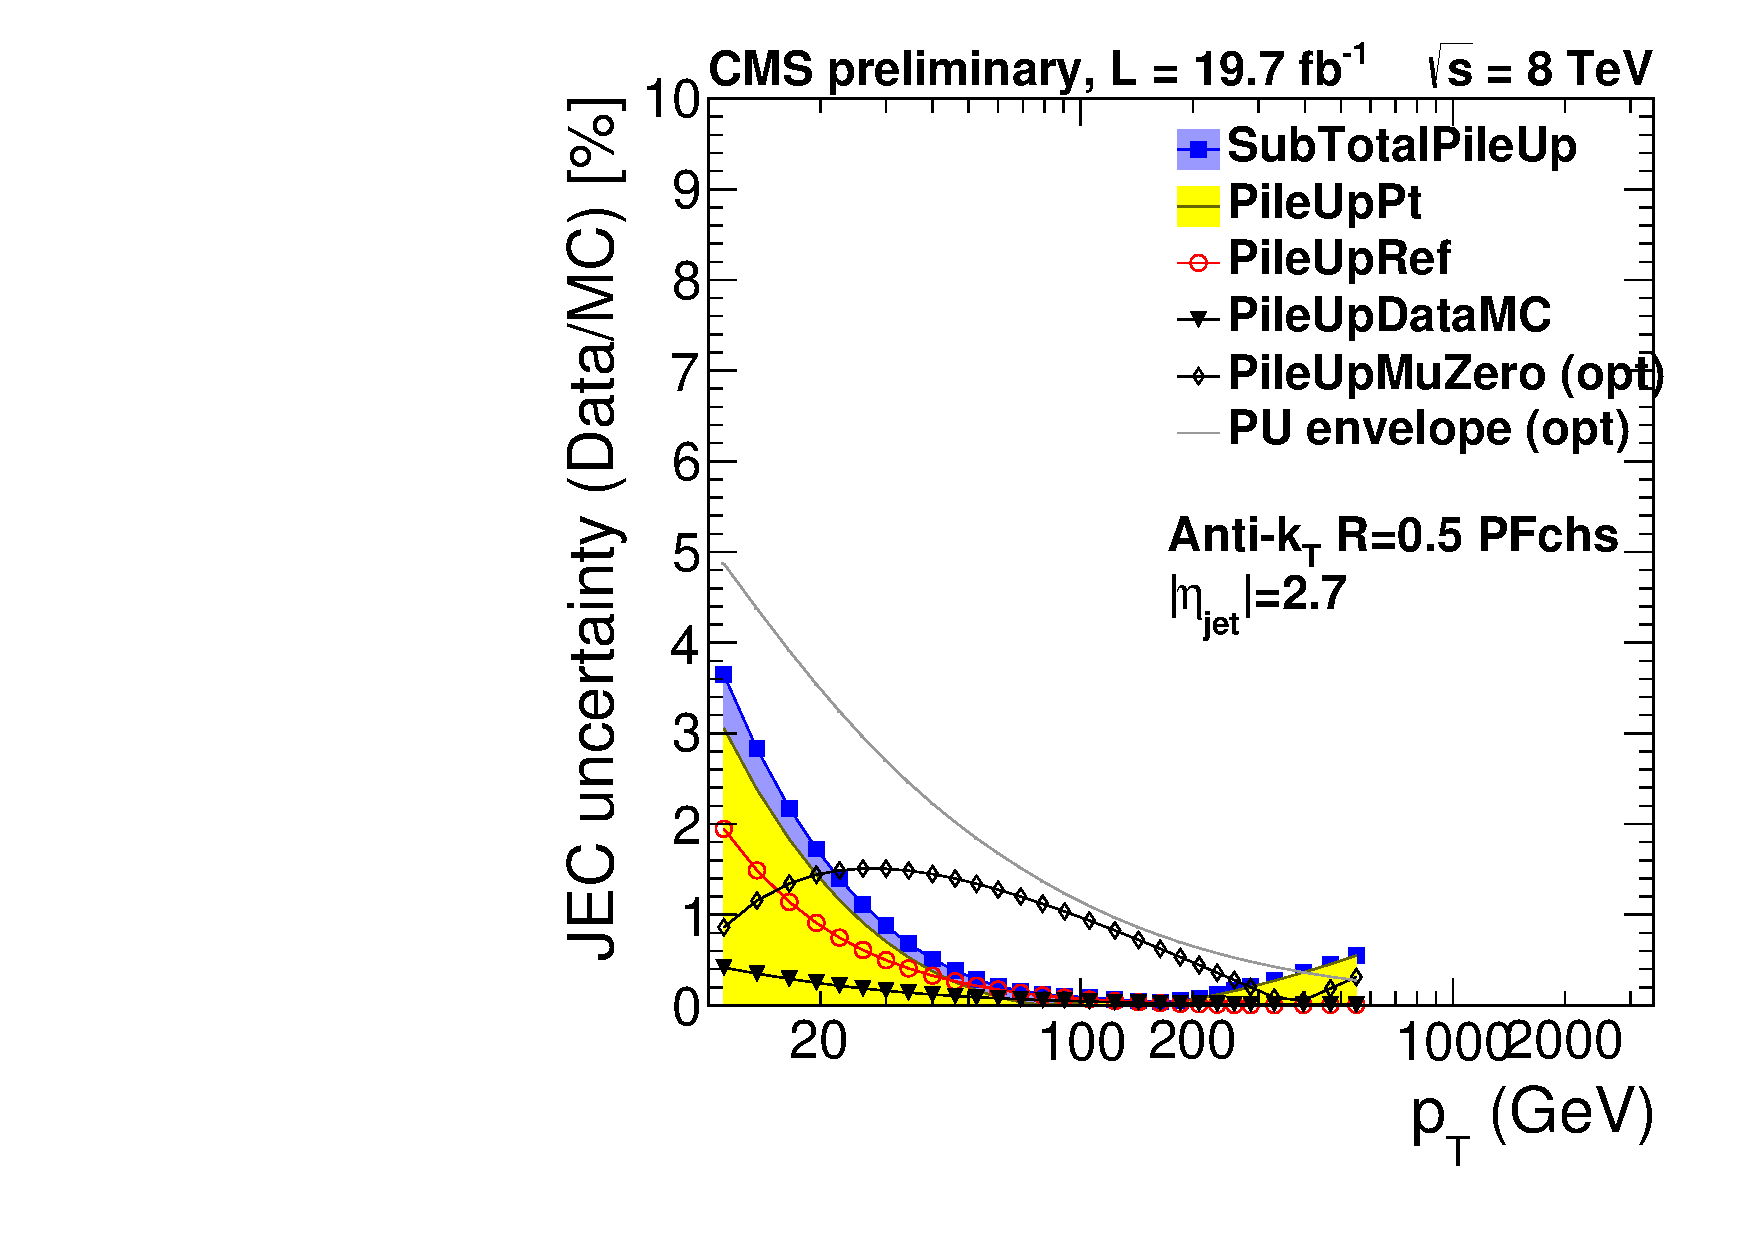
\includegraphics[width=0.25\textwidth]{images/JECUncert_PileUp_AK5PFchs_Eta27.pdf}%
			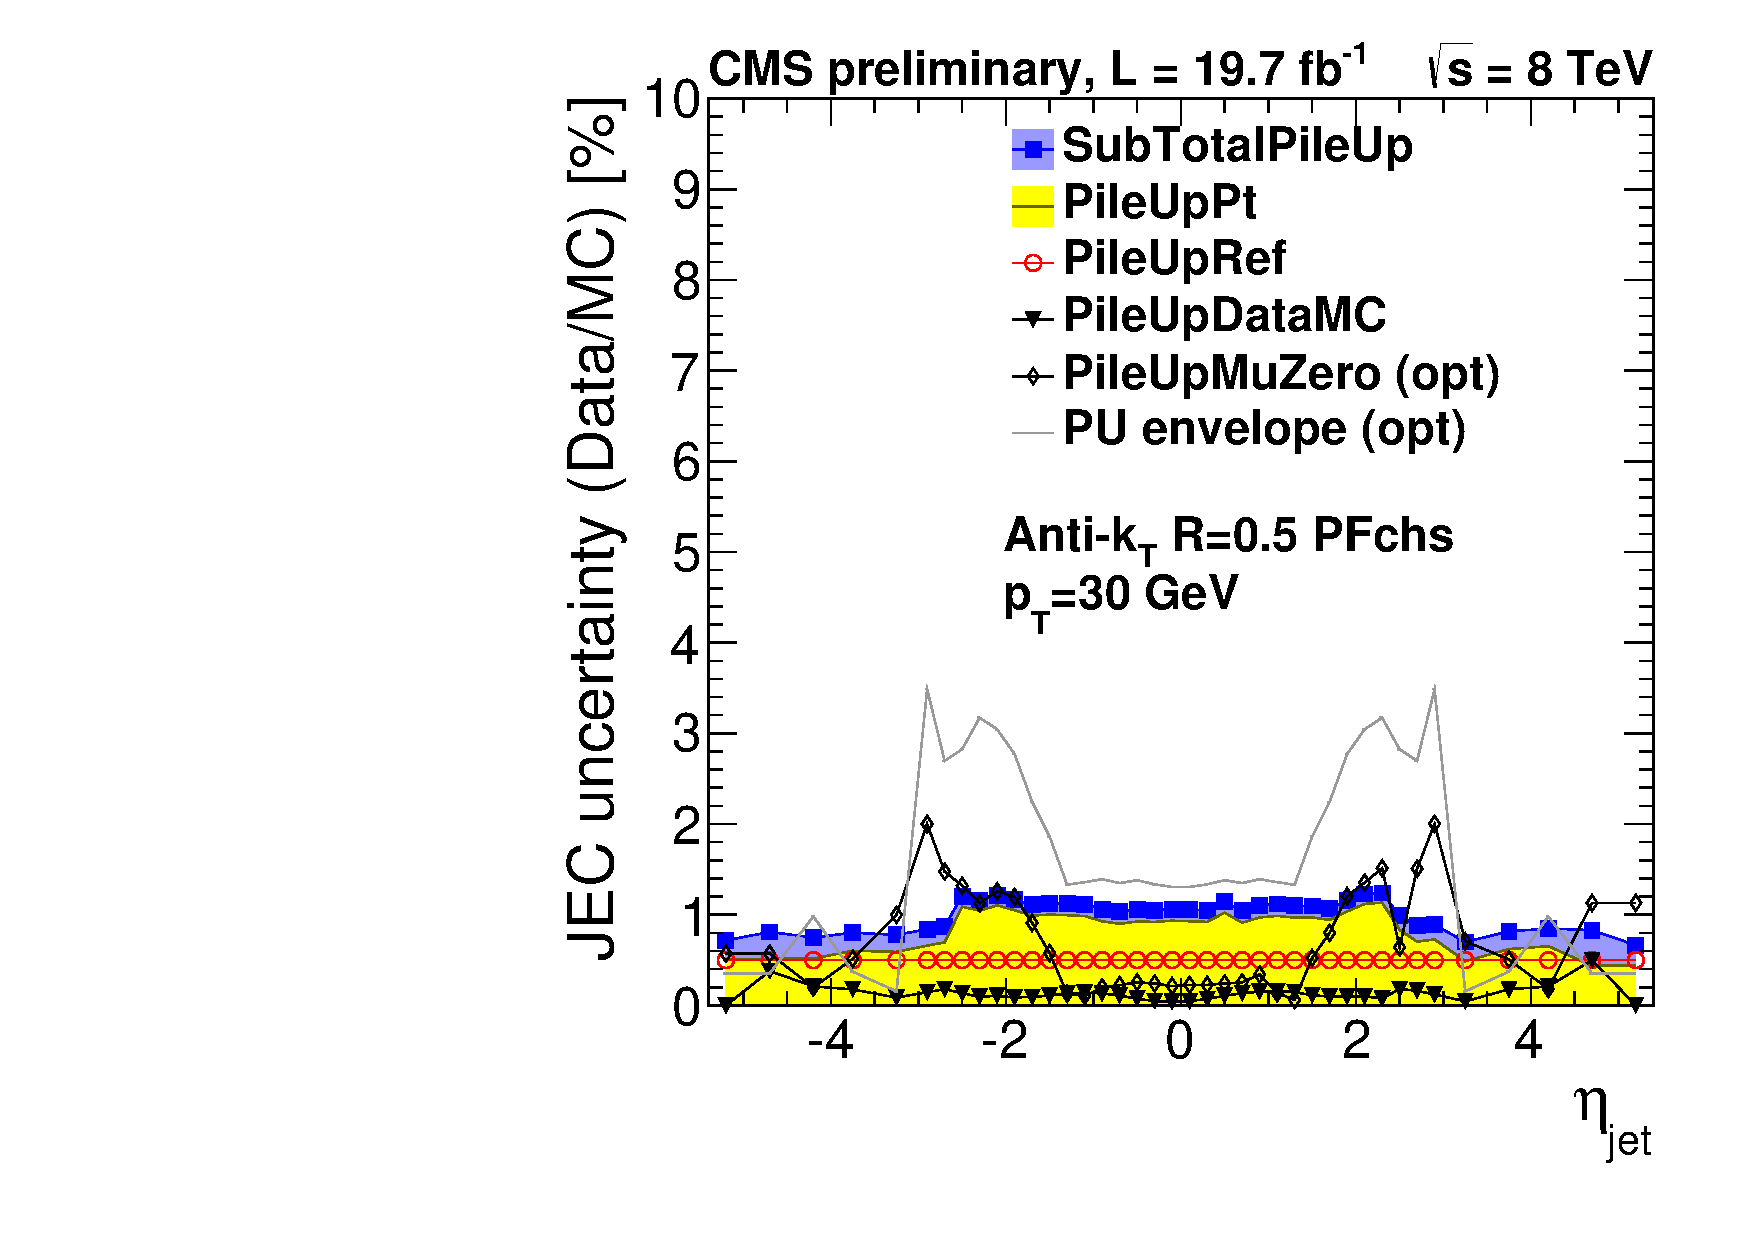
\includegraphics[width=0.25\textwidth]{images/JECUncert_PileUp_AK5PFchs_Pt30.pdf}%
			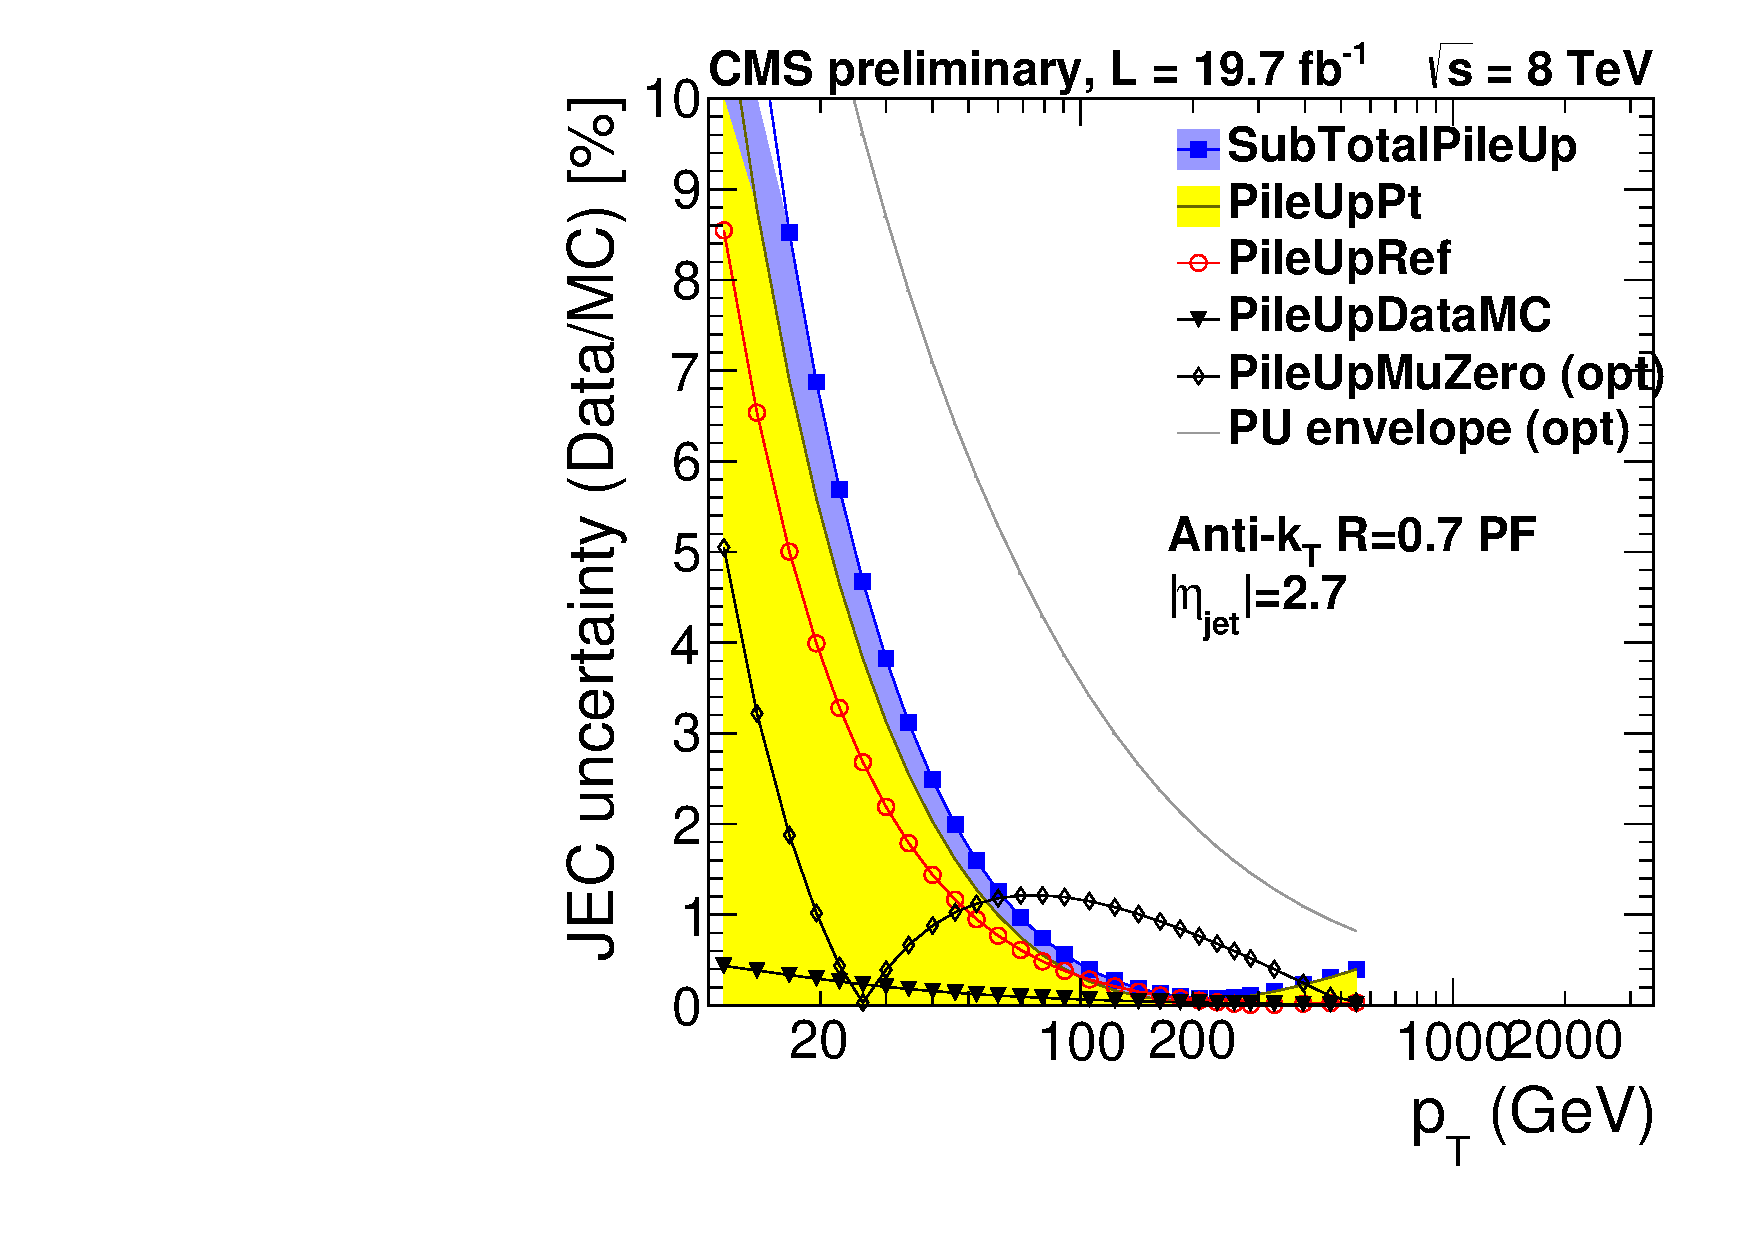
\includegraphics[width=0.25\textwidth]{images/JECUncert_PileUp_AK7PF_Eta27.pdf}%
			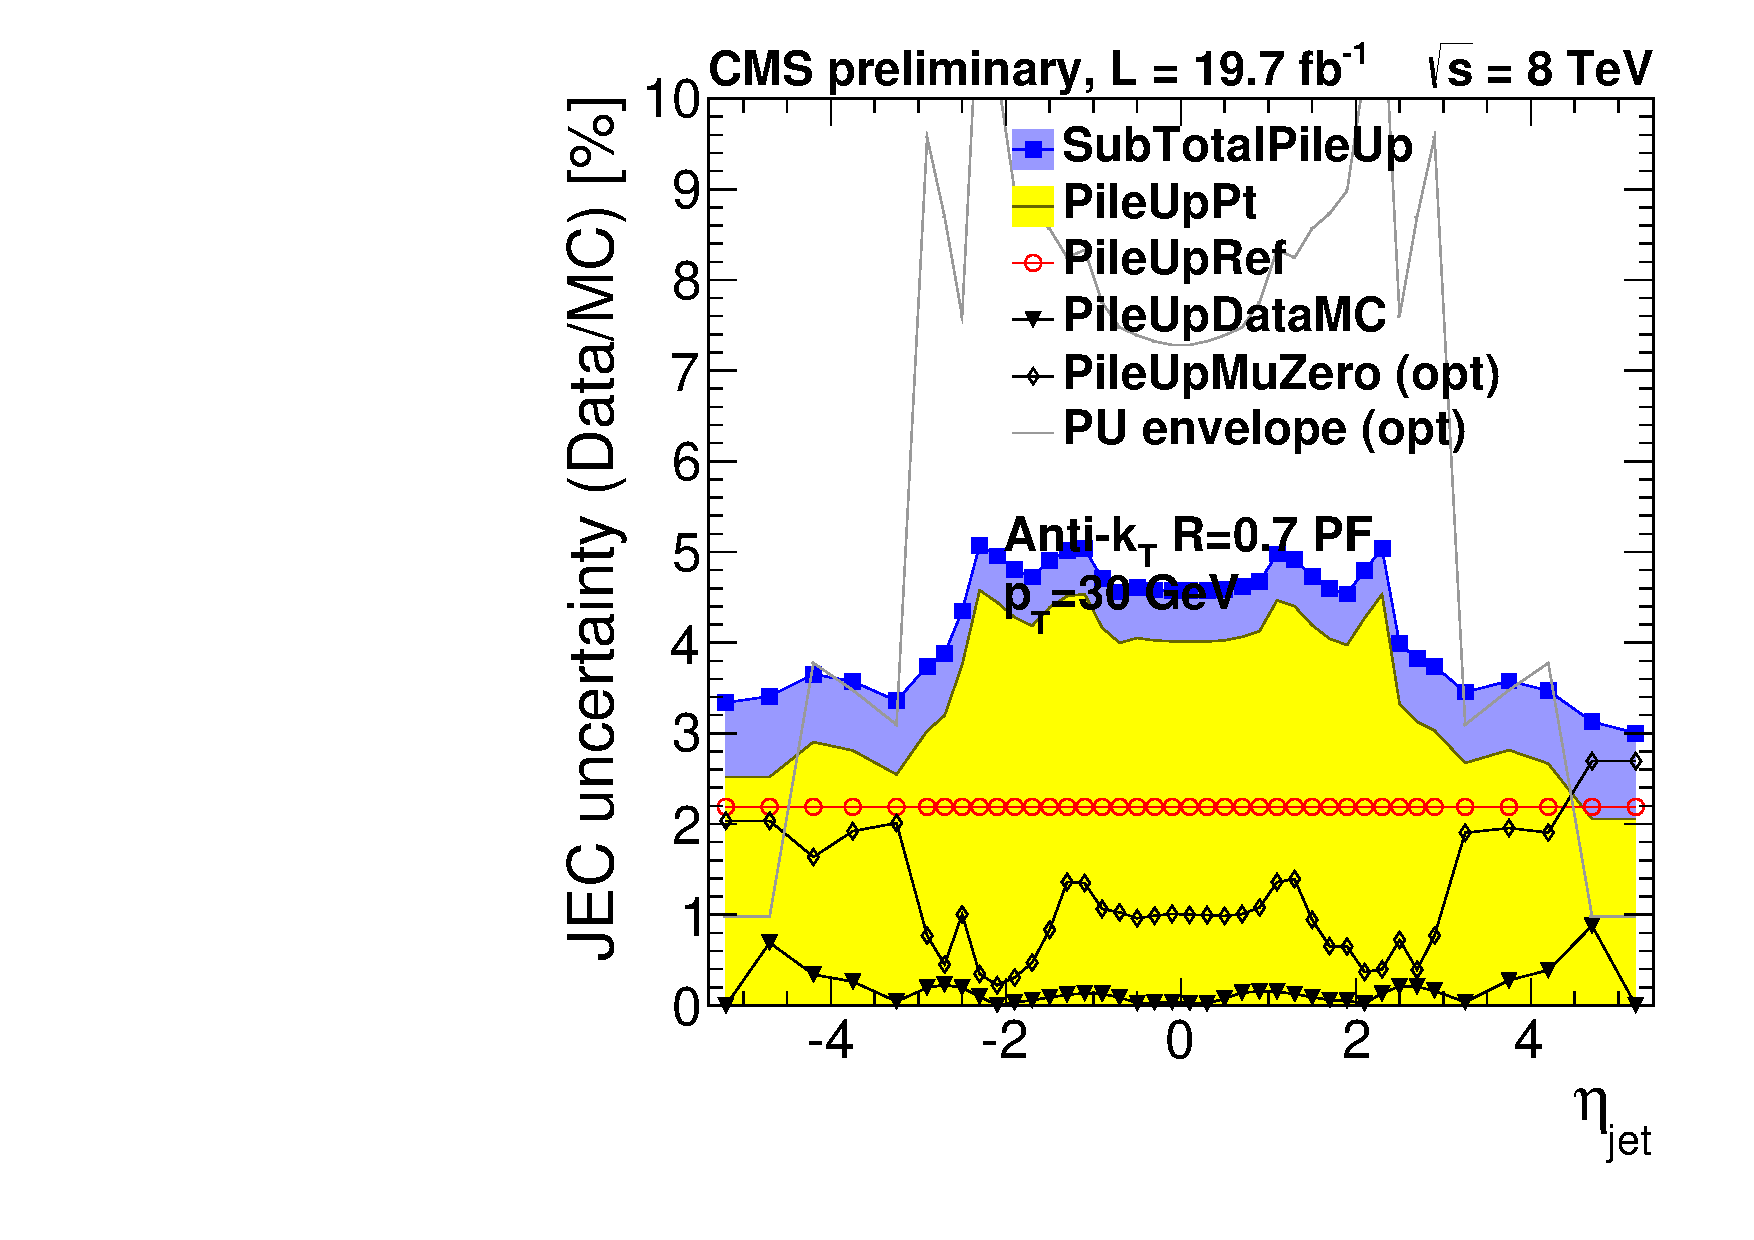
\includegraphics[width=0.25\textwidth]{images/JECUncert_PileUp_AK7PF_Pt30.pdf}%
		};
	\end{myfancyblock}
	
}
\subsection*{MuZero}
\frame{
	\frametitle{PileUpMuZero}
	\vspace*{-0.24cm}
	\begin{block}{}
		\begin{itemize}
			\item We compensate for the offset residual in L2L3Res for $<\mu>=20$
			\item This means it is biased for $<\mu>=0$
			\begin{itemize}
				\item $<\mu>=0$ is relevant for $2.76\unit{TeV}$ analyses
			\end{itemize}
			\item Have a new, optional systematic called PileUpMuZero
		\end{itemize}
	\end{block}
	\begin{myfancyblock}
		\node[anchor=south west,inner sep=0] (image) at (0,0) {%
			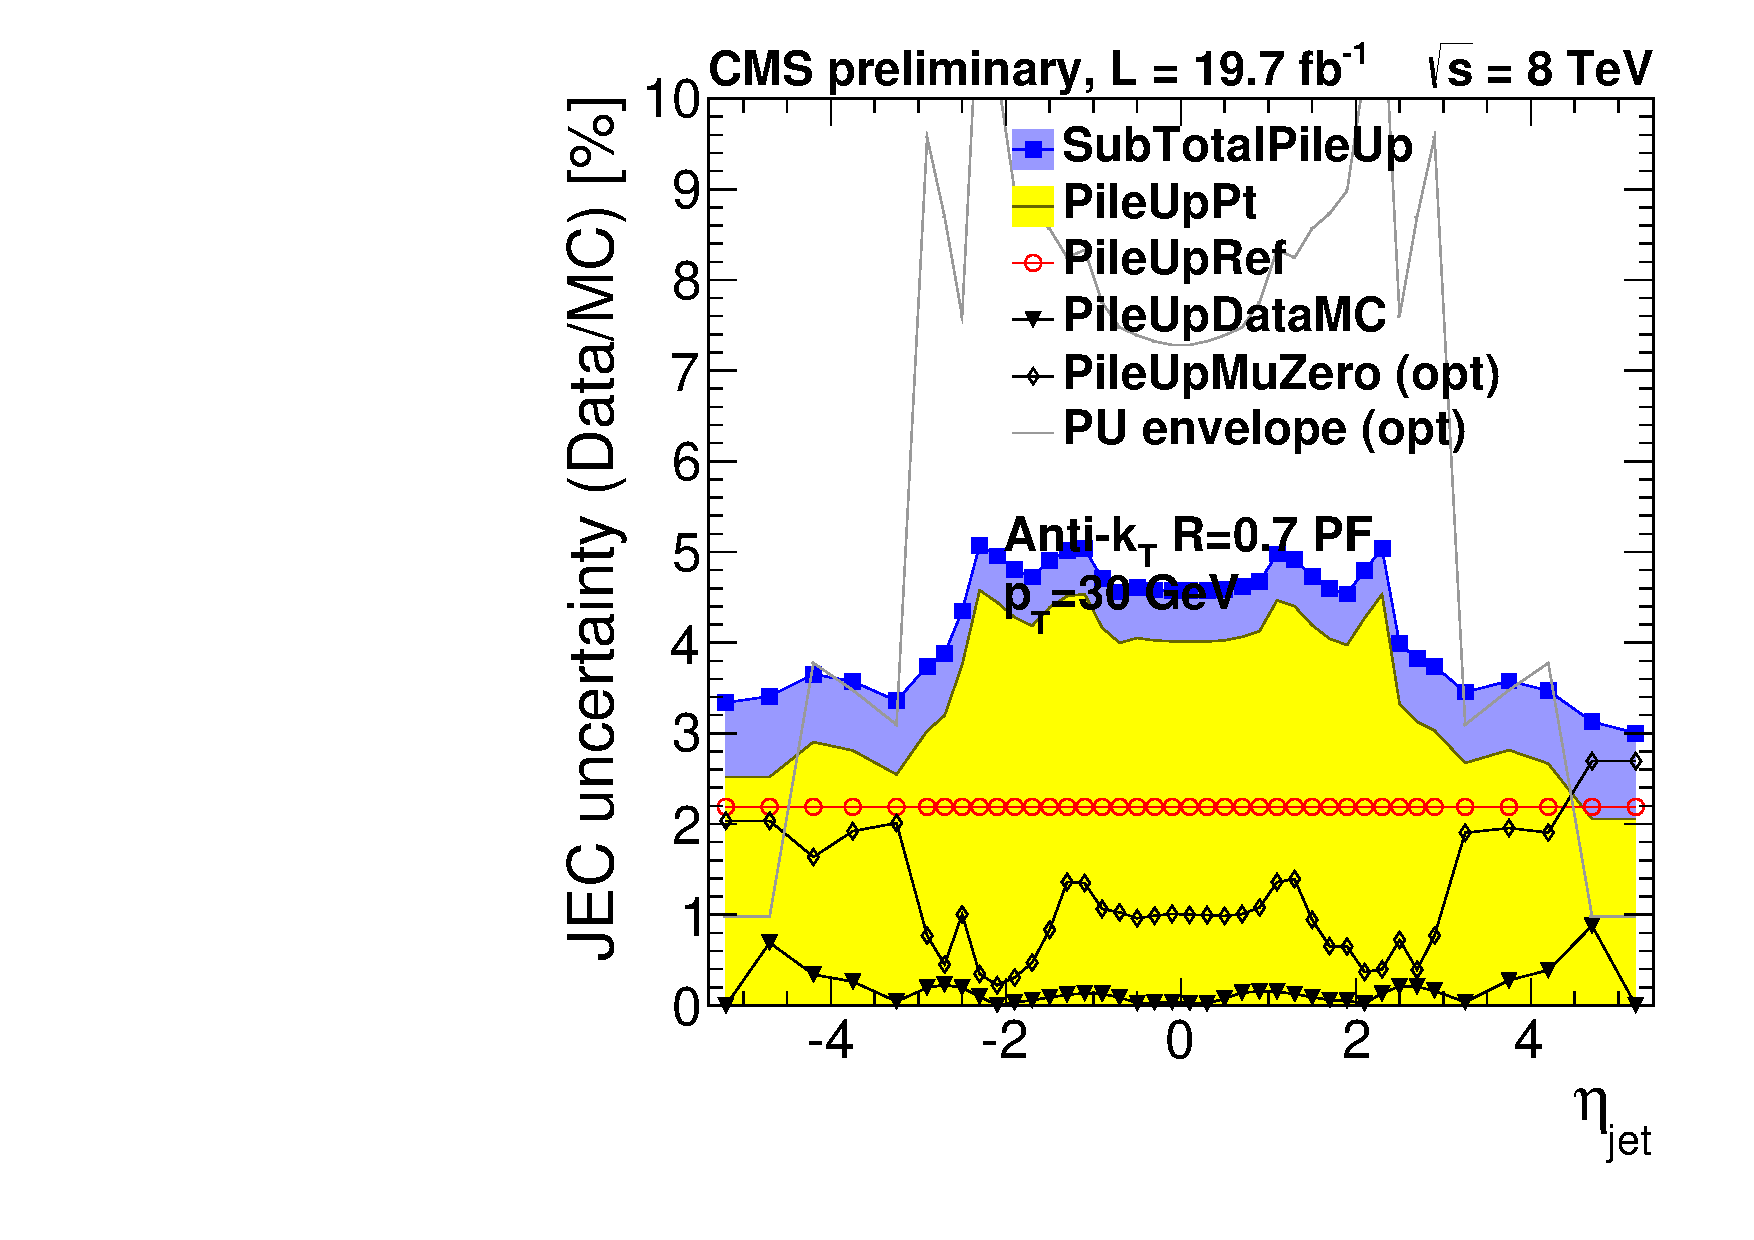
\includegraphics[width=0.46\textwidth]{images/JECUncert_PileUp_AK7PF_Pt30.pdf}%
			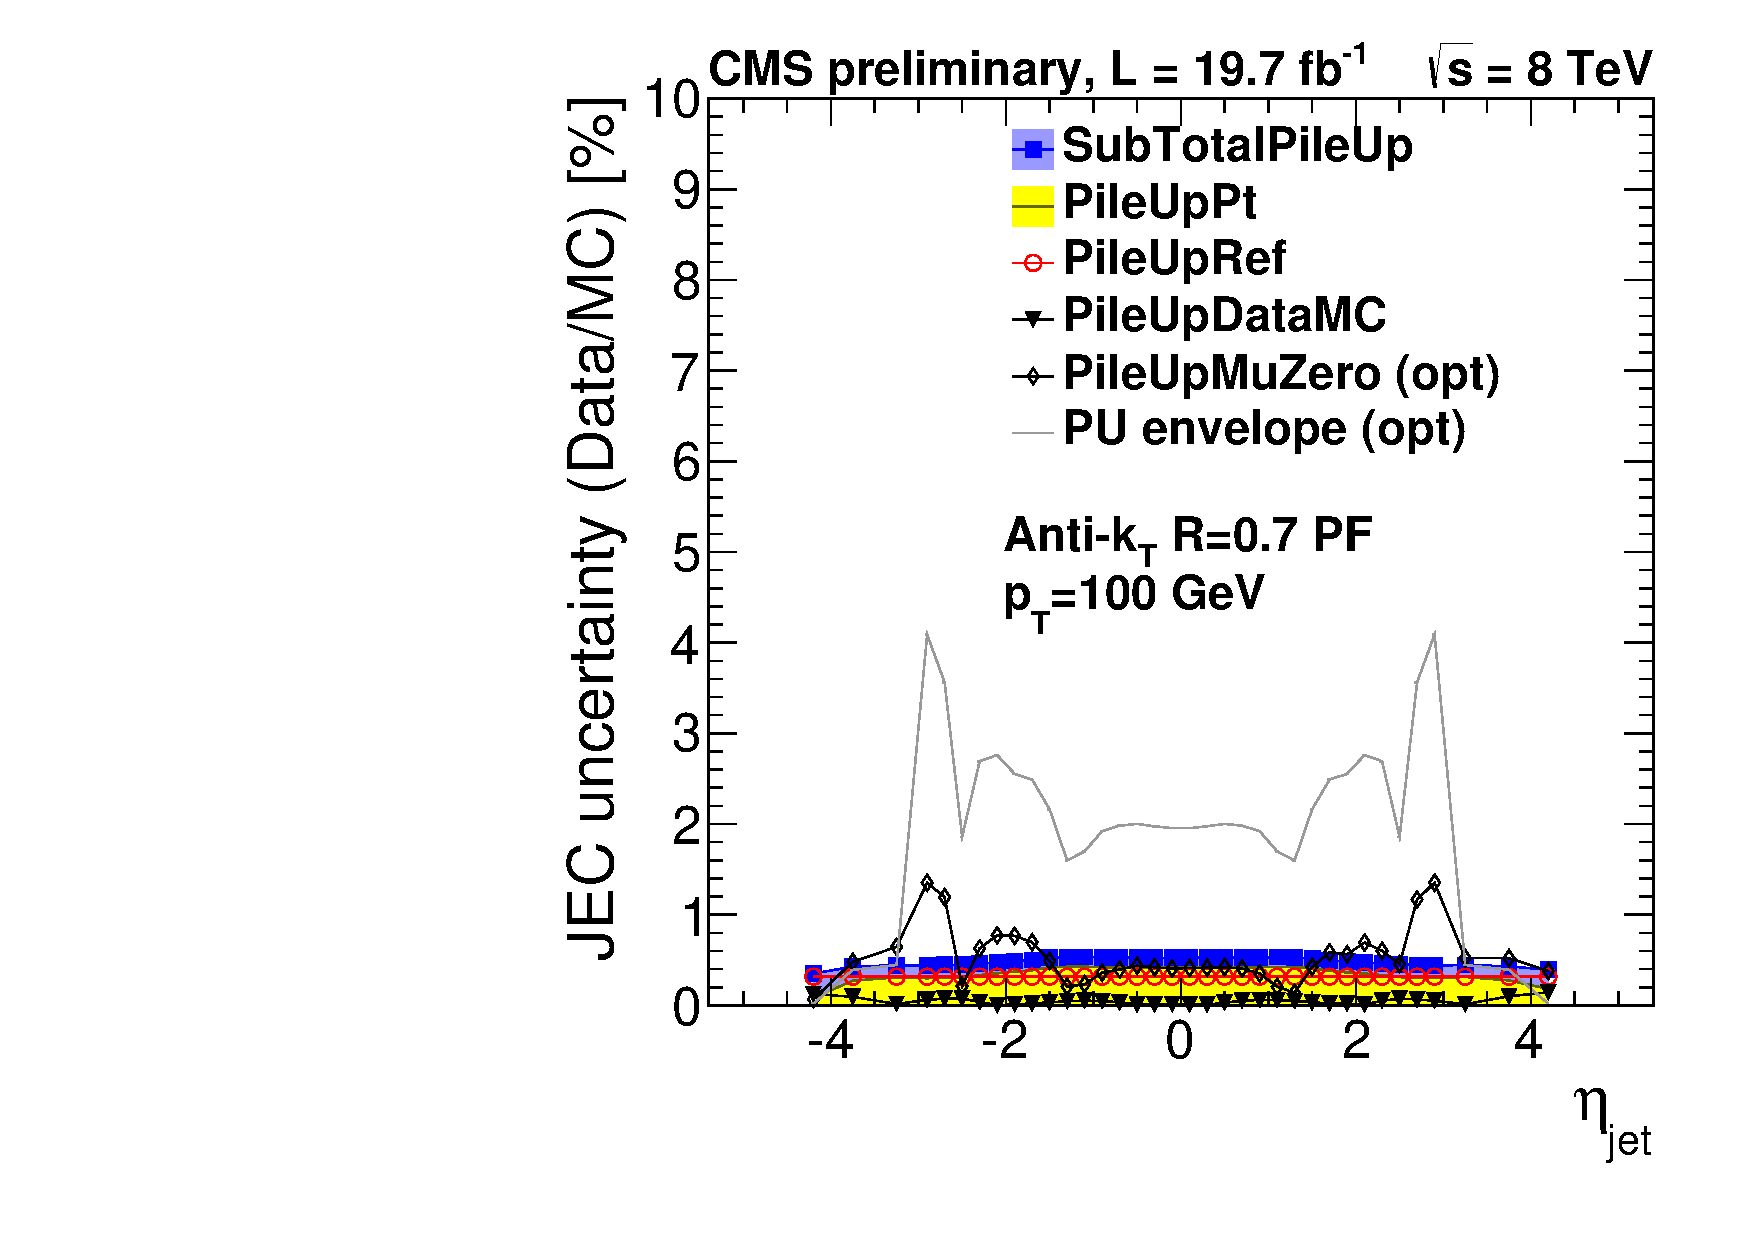
\includegraphics[width=0.46\textwidth]{images/JECUncert_PileUp_AK7PF_Pt100.pdf}%
		};
	\end{myfancyblock}
}
\subsection*{TimePt}
\frame {
	\frametitle{Time}
	\vspace*{-0.24cm}
	\begin{columns}[T]
	\column{0.64\textwidth}
	\vspace*{-0.3cm}
	\begin{block}{}
		\begin{itemize}
			\footnotesize
			\item Time dependence in barrel response observed by Matthieu Marionnaeu in E/p studies
			\item Folded into the TimePt systematic
			\item Special TimeRun[A,B,C,D] to estimate the effect for each run range
			\begin{itemize}
				\footnotesize
				\item Done by varying the single pion response by an amount corresponding to relative E/p change for $p_{T}>10\unit{GeV}$ hadrons
			\end{itemize}
			\item Specifically done for SMP-J, which reported the slope in the inclusive jet cross section changing with time
		\end{itemize}
	\end{block}
	\vspace*{-0.41cm}
	\begin{center}
	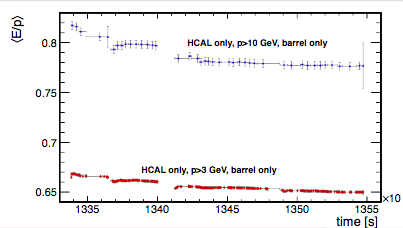
\includegraphics[width=0.8\textwidth]{images/Eop_BH_3_10.png}%
	\end{center}
	\column{0.34\textwidth}
	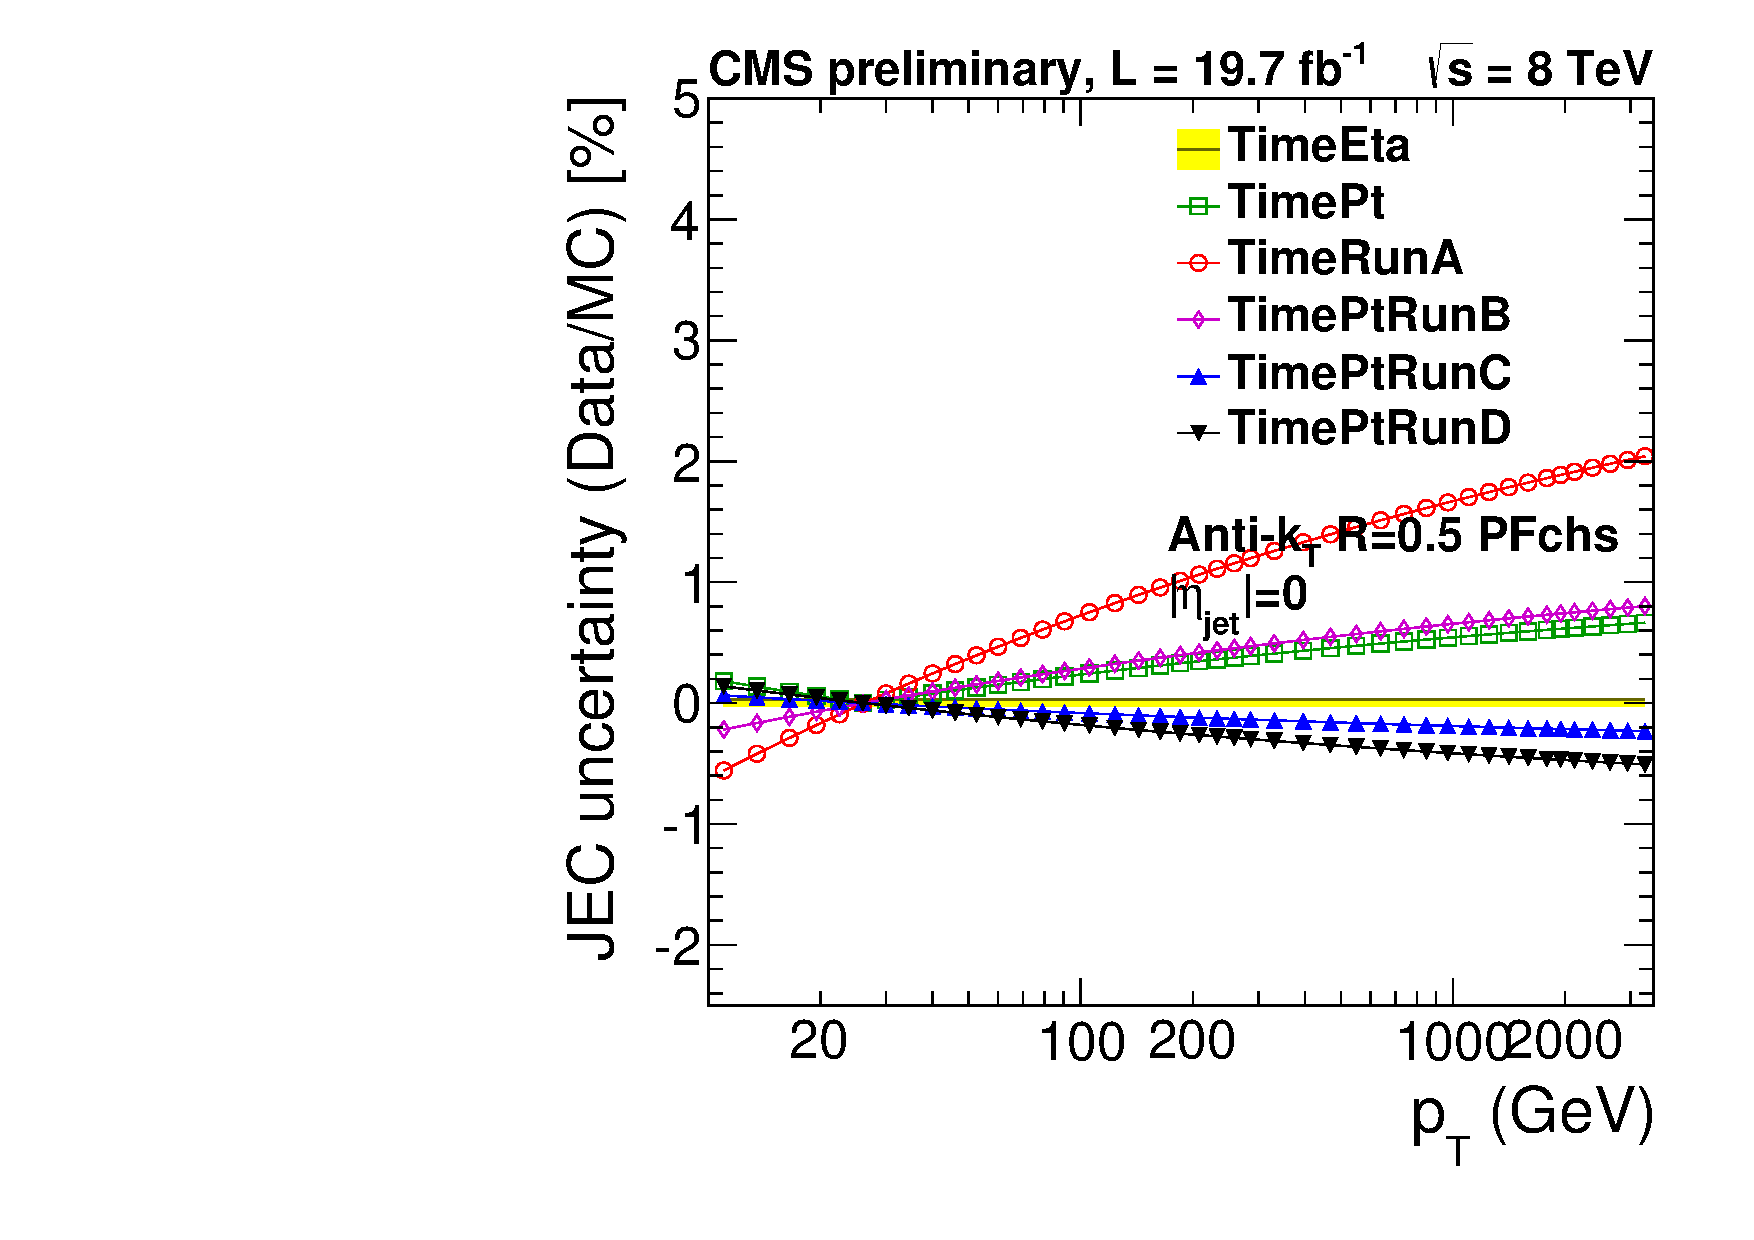
\includegraphics[width=\textwidth]{images/JECUncert_Time_AK5PFchs_Eta00.pdf}\\
	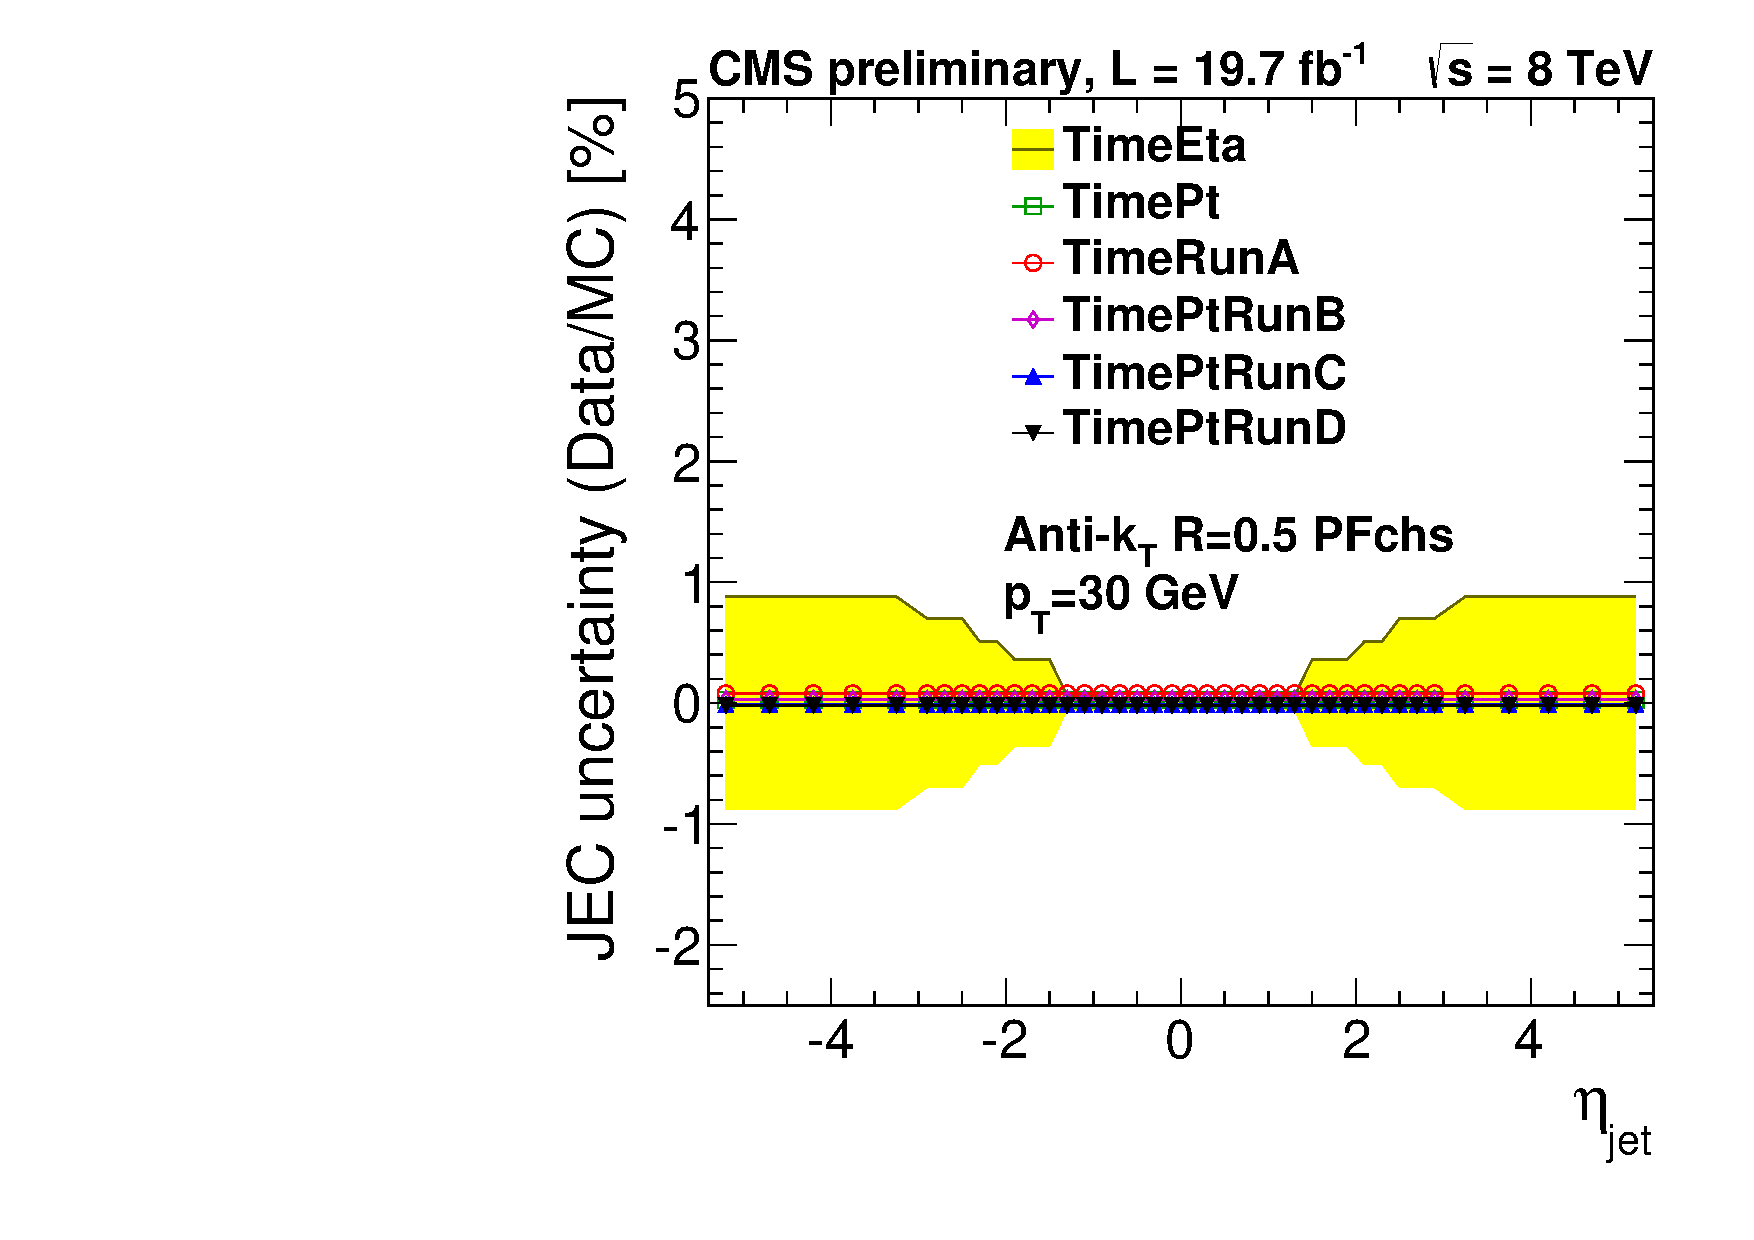
\includegraphics[width=\textwidth]{images/JECUncert_Time_AK5PFchs_Pt30.pdf}%
	\end{columns}
}